\documentclass[a4paper,12pt, openright]{report}

% links
\usepackage{hyperref}
% foreach macro
\usepackage{pgffor}
\usepackage{array}
\usepackage{subcaption}
\usepackage{graphicx}
\usepackage{amsmath}
\usepackage{bookmark}
\usepackage{tabularx}
\usepackage{longtable}
\usepackage{caption}
\usepackage{float}
\usepackage[italian]{babel}
\usepackage[T1]{fontenc}
\usepackage{bm}
\usepackage{newtxtext,newtxmath}
\usepackage{graphicx}
\usepackage{hyperref}
\usepackage[T1]{fontenc}
\usepackage[utf8]{inputenc}
\usepackage{setspace}
\usepackage[paper=a4paper,margin=1in]{geometry}
\usepackage{afterpage}
%\usepackage[nottoc,numbib]{tocbibind}


\setcounter{secnumdepth}{5}
\setcounter{tocdepth}{5}

\newcommand\blankpage{%
    \null
    \thispagestyle{empty}%
    \addtocounter{page}{-1}%
    \newpage}
\usepackage[
    left = \flqq{},% 
    right = \frqq{},% 
    leftsub = \flq{},% 
    rightsub = \frq{} %
]{dirtytalk}
\DeclareUnicodeCharacter{2212}{-}



\begin{document}
    
\begin{titlepage}
    \noindent
    \begin{minipage}[t]{0.19\textwidth}
        \vspace{-4mm}{
\includegraphics[scale=1.15]{logo_unimib.pdf}}
    \end{minipage}
    \begin{minipage}[t]{0.81\textwidth}
        \setstretch{1.42}
        \textsc{Università degli Studi di Milano - Bicocca} \\
        \textbf{Scuola di Economia e Statistica} \\
        \textbf{Dipartimento di Statistica e Metodi Quantitativi} \\
        \textbf{Corso di laurea in Statistica e Gestione delle Informazioni} \\
        \par
    \end{minipage}
    \vspace{40mm}
    \begin{center}
        \large \setstretch{1.2}
        \textbf{Competitività in Europa \\ Una analisi multidimensionale tra stati}
        \par
    \end{center}
    \vspace{50mm}
    \noindent
    {\large \textbf{Relatore:} Prof. Fattore Marco} \\
    \vspace{15mm}
    \begin{flushright}
        {\large \textbf{Relazione di:}} \\
        \large{Jimenez Iris Dania} \\
        \large{Matricola 827147}
    \end{flushright}
    \vspace{40mm}
    \begin{center}
        {\large{\bf Anno Accademico 2021-2022}}
    \end{center}
    \restoregeometry
\end{titlepage}


\newpage
    

\begin{center}
    \chapter*{\centering Prefazione}
    Mi sono imbattuta nell'argomento dei Poset(\textit{Partially ordered set}) durante le lezioni del Prof. Fattore Marco, relatore di questa tesi. Sono rimasta 
    colpita ed affasciata da questo diverso approccio ai dati e all'analisi matematico-statistica, che si discosta dai metodi tradizionali. Ho così deciso di 
    approfondire lo studio di questo argomento, applicandolo anche al mondo che ci circonda ed in cui viviamo, l'Europa. 
\end{center}

\afterpage{\blankpage}

%\chapter*{Ringraziamenti} %allinea a destra 
\newpage
%\cleardoublepage
\begingroup
\let\clearpage\endgroup
%\null\vspace{\stretch{1}}
\chapter*{\centering Ringraziamenti}
\begin{flushright}
    \textit{
        A mia mamma, mio fratello e mio papà per essere la mia famgilia e avermi sempre sostenuto, \\
        Ad Adrian, per farmi essere una persona migliore, \\
        A Sofia, la mia sorella dalle stelle, \\
        A mi abuela Isabela e a nonna Iole per avermi cresciuta, \\
        \vspace{5mm} %5mm vertical space
        Per aspera ad astra.
    }

\end{flushright}

\newpage

\begin{center}
    \chapter*{\centering Abstract}
    Convenzionalmente, i dati di tipo ordinale sono stati visti come di livello in qualche modo inferiore rispetto ai più studiati
    dati numerici. In particolar modo, basti pensare come, per molti concetti esprimibili in modo unicamente ordinale si tende a credere che 
    la “variabile latente” vera, che sottosta all’indicatore ordinale, sia di tipo numerale e l’indicatore ordinale sia 
    solo un’espressione di questo numero. Questa linea di pensiero ha portato gli sforzi 
    matematico-statistici a concentrarsi su tecniche principalmente applicabili a dati di tipo numerico, 
    tralasciando i dati non numerici. \\
    Negli ultimi anni però, i dati di tipo ordinale sono sempre stati maggiormente impiegati ed utilizzati, sia perchè in campo 
    sociale molti concetti sono esprimibili in questo formato sia perchè, sono state sviluppate nuove tecniche 
    specifiche per i dati ordinali. 
    I Poset(\textit{Partially ordered set}) appartengono proprio a quest’ultima categoria e formalizzano e generalizzano il 
    concetto di ordinamento e comparazione. Essi, quindi, permettono di analizzare insieme di indicatori ordinali, 
    tenendo conto proprio della loro natura non numerica. \\ In questa tesi, i Poset verranno utilizzati per creare una 
    classifica in diversi ambiti dei vari stati europei, inoltre sempre tramite i poset verrà creato un punteggio di
    incomparabilità tra stati, che andrà a tenere conto di quanto, in un ranking, i punteggi siano affidabili. 
    Quest'ultima informazione viene spesso trascurata, eppure risulta essere estremamente importante perchè, 
    anche se è vero che le classifiche ci aiutano a comprendere meglio la realtà, dobbiamo sempre tenere conto che quella che abbiamo davanti è una sintesi, 
    una forzatura, e che i numeri che vediamo non sono sempre così semplicemente interpretabili.  
\end{center}

\afterpage{\blankpage}


\tableofcontents





\newpage



\afterpage{\blankpage}

\chapter{Introduzione}

In questa tesi si è sviluppato il concetto di \say{competitività} tra diversi stati, a partire dal European Innovation Scoreboard(EIS),
con lo scopo di creare una classifica dei paesi europei più competitivi in diversi settori, per poterli comparare tra di 
loro in modo tale da considerare nella 
lettura dei risultati anche 
le differenze 
che esistono tra diversi stati.  
L'EIS è un dataset, pubblicato ogni anno a partire dal 2014 dall'Unione Europea, composto da un insieme di indicatori che 
valutano 
le performance sotto diversi punti di vista dei vari stati Europei.  \\
\\
Il World Economic Forum definisce la competitività tra paesi come \linebreak
$\textit{\say{l'insieme di istituzioni $\newline$ e politiche che determinano 
il livello di produttività $\newline$ di un paese}}$[1], \\ mentre The Oxford Dictionary la definisce come  \linebreak
$\textit{\say{l'abilità di un'economia di aumentare la domanda e mantenere alte le esportazioni}}$[2]. \\
Entrambe queste definizioni non sono molto precise, in quanto non individuano quali siano i fattori determinanti che contribuiscono a 
formare la competitività di un paese, ma invece indicano delle metriche per cercare di misurarla, come la produttivà e il livello 
di esportazioni di un paese. Inoltre, entrambe queste definizioni si concentrano fortemente sull'aspetto economico della competitività di un paese, tralasciando altri fattori. Intuitivamente 
quando pensiamo ad un paese \say{competitivo}, la sfera economica risulta essere certamente importante e determinante nel 
definire il livello di competitività di uno stato, ma non è l'unico aspetto da considerare. Vi sono, infatti, altri fattori che
influiscono sul concetto di \say{competitività}, i quali però non risultano essere altrettanto discussi e analizzati dalle 
istituzioni.  \\
Con questa tesi il mio obiettivo invece è quello di sviluppare il concetto di \say{competitività} con lo scopo di indivuare quali sono i 
fattori che la determinano e che la influenzano, utilizzando gli indicatori presenti nel European Innovation Scoreboard, per infine 
creare una classifica dei diversi stati europei che mostri quali sono i paesi più \say{competitivi}. In aggiunta, si svilupperà anche il concetto di \say{incomparabilità}, ossia di come di fronte ad una classifica, quanto possiamo porre a confronto i punteggi ottenuti 
da due differenti stati. Questa nozione aiuta anche a tenere sempre presente che i valori che si vogliono comparare non sono dei semplici numeri, ma esprimono 
concetti più profondi, non sempre facilmente identificabili da una nozione di \say{migliore} e \say{peggiore}.\\
Una classifica multidimensionale sulla competitività può aiutare le istituzioni a comprendere quali sono gli elementi che la determinano e 
che la influenzano, andando così a fornire un supporto nel capire quali sono i settori ed i paesi che maggiormente necessitano di 
aiuti e finanziamenti per aumentare la loro competitività a livello europeo. \\
Queste informazioni possono fornire validi ed efficaci insights con il fine di avvantaggiare e favorire i paesi europei a livello 
internazionale, sotto un'ottica di cooperazione e solidarietà tra stati membri, tenendo però sempre conto delle caratteristiche che compongono i singoli stati.\\
\\
Prendendo in considerazione più dimensioni, oltre a quella prettamente economica, risulta assai più complesso e meno intuitivo creare
una classifica della \say{competitività} tra paesi, questo perchè alcuni stati potrebbero avere performance maggiori su alcune dimensioni e minori 
su altre, andando così a creare contrasti difficilmente risolvibili. Date queste complessità ho utlizzato la teoria degli ordinamenti parzialmente ordinati(poset), che ha proprio lo scopo di formalizzare e 
generalizzare il concetto di \say{ordinamento}. I poset sono $\textit{parzialmente ordinati}$ perchè non ogni coppia di elementi è 
comparabile, ossia vi sono delle incomparabilità, come nel caso in cui un paese abbia dei valori maggiori su alcuni indicatori e minori 
su altri, ma nonostante queste difficoltà gli ordinamenti parzialmente ordinati sono in grado di fornire un ordinamento
$\textit{totalmente ordinato}$, in cui ogni coppia di elementi, stati nel nostro caso, è comparabile. \\
Nella seconda sezione di questa tesi descriverò la teoria degli ordinamenti parzialmente ordinati e spiegherò come, nonostante 
sussistano delle incomparabilità tra gli elementi di un dataset, i poset sono in grado di fornire comunque un unico ordinamento finale e di come si possa anche 
ricavare un punteggio di \say{incomparabilità}. Successivamente 
presenterò i dati utilizzati e descriverò le principali tecniche statiche e computazionali utilizzate nell'analisi dei dati. Infine 
presenterò i risultati e le conclusioni delle analisi. 




\newpage


\chapter{Insiemi parzialmente ordinati}

I poset(partially ordered set) sono insiemi parzialmente ordinati utilizzati in matematica, in 
particolare nella teoria degli ordini, 
per effettuare una riduzione della dimensionalità su dati di tipo ordinale. Lo scopo dei poset quindi,
risulta essere quello di ridurre ad un ranking, ossia una struttura di tipo unidimensionale, un insieme di indicatori ordinali 
i quali si presentano come degli oggetti multidimensionali. \\
Gli indicatori di tipo ordinale sono ampiamente diffusi sopratutto in campo sociale e vengono 
utilizzati per esprimere idee e nozioni che per loro natura non posso essere rigorosamente ordinate secondo 
una scala metrica. Per esempio, i concetti legati alla sfera emotiva come la felicità, la soddisfazione ed il benessere vengono espressi tramite indicatori di questo tipo, inoltre appartengono alla famiglia dei dati ordinali 
tutti quegli indicatori che richiedono di esprimere un giudizio o un'opinione.\\
Il problema che si incontra con questo tipo di dati è quello di effetturare un'analisi statistica
multivariata su un tipo di dato \say{non-matematico}. Per ovviare a questo problema molto spesso si 
cerca di trasformare in una qualche maniera il dato ordinale in un dato numerico, per poi procedere 
con le usuali tecniche di analisi statistica che meglio si conciliano con i fini della ricerca. \\
Tralasciando il discorso su che tipo di risultati le canoniche tecniche di analisi possono 
produrre su dati la cui vera natura è non numerica, il problema che si pone è un altro e di natura 
ben più profonda; perchè dover necessariamente trasformare il dato? Questa idea si basa sul concetto 
che la forma in cui il dato viene naturalmente espresso sia in qualche modo sub-ottimale e di minor 
qualità rispetto al classico dato numerico. Eppure nella nostra quotidiana esperienza tutti noi facciamo
largamente uso di questo tipo di dato; nella vita di tutti i giorni non esprimiamo i concetti e le nostre esperienze
in numeri ma tramite le nozioni di \say{migliore} o \say{peggiore}, \say{buono} e \say{meno buono}, \say{bello} e \say{brutto}. 
Perchè allora cercare di forzare e trasformare la vera natura del dato? Perchè assumere che la vera 
variabile latente sottostante al concetto che vogliamo esprimere sia numerica? Soprattutto, alla luce di 
questi nuovi concetti sarebbe ancora ragionevolmente sensato e attendibile 
interpretare come veritiero ciò che otteniamo come risultato? \\
Un nuovo e differente approccio è quello di cercare di mappare i dati come sono senza trasformazioni, 
ed è in questo campo che vengono utilizzati i poset. Tramite la teoria degli ordinamenti parzialmente
ordinati si cerca di costruire una grammatica del dato multidimensionale che preservi la natura 
ordinale dello stesso. 

\section{Definizione}

Di seguito viene fornita la definizione standard di poset. \\
\\
Sia X un insieme e sia $\leq$ una relazione binaria, tale che abbia le proprietà di;\\
\\
1) Riflessività: x $\leq$ x, $\forall$ x $\in$ X\\
\\
2) Antisimmetria: x $\leq$ y e y $\leq$ x $\Leftrightarrow$ x = y, $\forall$ x, y $\in$ X \\
\\
3) Transitività: x $\leq$ y e y $\leq$ z $\Rightarrow$ x $\leq$ z, $\forall$ x, y, z $\in$ X\\
\\
Allora la coppia (X, $\leq$) è chiamata insieme parzialmente ordinato. \\
Un poset si presenta quindi come une relazione binaria tra un insieme X e la relazione d'ordine 
$\leq$  con le proprietà sopraelencate di riflessività, antisimmetria e transitività.\\
La proprietà di riflessività ci garantisce che ogni elemento è relazionato con se stesso, 
mentre la proprietà di antisimmetria assicura che qualunque siano gli elementi di x e y 
appartenenti all'insieme X, le relazioni  x $\leq$ y e y $\leq$ x non possono sussistere 
contemporaneamente quando x è diverso da y. Infine la proprietà di transitività afferma che 
se sussite una relazione tra x e y e, a sua volta, sussiste una relazione tra y e z, allora 
esisterà anche una relazione tra x e z, con x, y e z appartenenti allo stesso insieme X. 



\section{Diagramma di Hasse}

I poset possono essere rappresentati graficamente tramite il diagramma di Hasse, il quale prende il nome 
dal sui ideatore Helmut Hasse$\footnote[1]{Helmut Hasse fu un matematico tedesco che lavorò nel campo della teoria
algebrica dei numeri, fondamentali sono i suoi contributi alla teoria dei campi[3].}$(1898-1979). Esso si presenta come un grafo formato
 da un insieme di nodi uniti da archi orientati. Di seguito è riportato un esempio di un diagramma di Hasse. \\
 Sia P = (\{a, b, c, d, e, f, g, h, i, l\}, $\leq$) un insieme parzialmente ordinato. Un possibile diagramma di Hasse 
 associato può essere, il seguente; \\
 \begin{figure}[H]
    \centering
    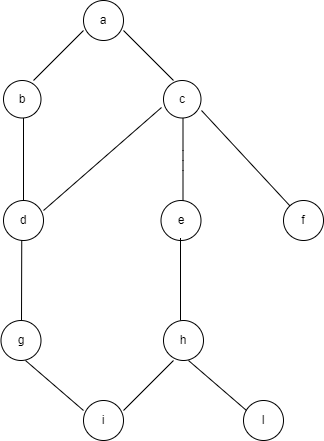
\includegraphics[scale=.5]{diagramma_hasse.png}
    \caption{Diagramma di Hasse del poset P}
\end{figure}

Il diagramma si legge dall'alto verso il basso e due generici elementi sono tra loro comparabili se 
risultano essere uniti da una sequenza discendente di archi; nel caso in cui questa sequenza discendente di 
archi non dovesse essere presente i due elementi sono incomparabili. \\
Nell'esempio proposto nella Figura 2.1 gli elementi \say{a} e \say{b} sono comparabili, mentre \say{b} e \say{f} sono incomparabili, 
in quanto non vi è una sequenza discendente di archi ad unire questi due elementi. \\
Tramite questa lettura il poset può essere interpretato come un insieme di coppie di elementi che possono
essere tra loro comparabili o non comparabili. \\
Ai fini di comprendere appieno il diagramma di Hasse è necessario introdurre un ulteriore concetto
di fondamentale importanza per gli ordinamenti parzialmente ordinati; la nozione di copertura. \\
\\
L'idea sottostante alla relazione di copertura è che un elemento $\textit{domina}$ un'altro elemento se e solo se vi è
una successione di \say{coperture} che lega i due elementi. Nell'esempio in Figura 2.1 \say{a} copre \say{b} perchè
\say{sta sopra} a quest'ultimo. A sua volta \say{b} domina \say{d} e per la proprietà di transitività \say{a} 
domina a sua volta \say{d}. Si formano così insiemi di coppie comparabili o incomparabili, ed in tal senso possiamo dire che la relazione 
di copertura genera la relazione d'ordine, dato che quest'ultima è ottenuta seguendo transitivamente gli archi che collegano i punti. \\
Quando un elemento domina tutti gli altri assume il nome di $\textit{massimo}$. In Figura 2.1 \say{a} è un massimo, appunto perchè
domina tutti gli altri elementi. Nel diagramma di Hasse soprarappresentato, non sono presenti $\textit{minimi}$, in quanto nessun elemento viene dominato
da tutti, ma sono invece presenti dei $\textit{minimali}$, elementi che non dominano nessuno ma non sono dominati da tutti. 
Nell'esempio illustrato precedentemente i minimali risultano essere gli elementi \say{f}, \say{i} ed \say{l}. \\
Una rappresentazione di un diagramma di Hasse in cui sono presenti $\textit{minimi}$ e $\textit{massimali}$, è la seguente;\\
\begin{figure}[H]
    \centering
    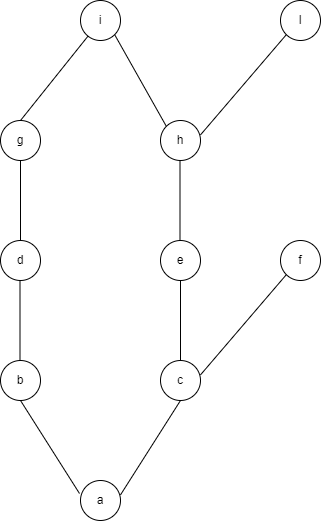
\includegraphics[scale=.5]{hasse2.png}
    \caption{Diagramma di Hasse del poset P}
\end{figure} 

Nella Figura 2.2 l'elemento \say{a} è un minimo, perchè viene dominato da tutti gli elementi, mentre \say{i}, \say{l}, \say{f} sono dei massimali,
in quanto non vengono dominati da nessuno ma non dominano tutti. \\
Un poset con un numero finito di elemento ammette sempre minimali e massimali, ma non sempre ha massimo o minimo. \\
\\ 
In un insieme parzialmente ordinato un sottoinsieme di elementi tutti fra loro comparabili viene chiamato $\textit{catena}$.
Nella Figura 2.3 un esempio di catena è dato dal sottoinsieme composto dagli elementi \say{a}-\say{b}-\say{d}-\say{g}-\say{i}\\
\begin{figure}[H]
    \centering
    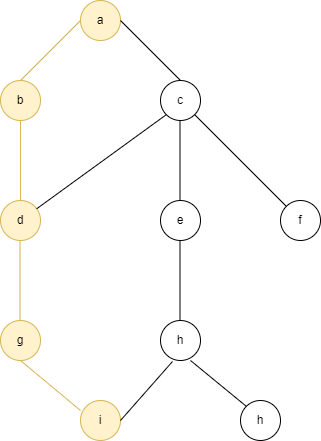
\includegraphics[scale=.5]{hasse_catena.png}
    \caption{Evidenziata una catena}
\end{figure}

Le anticatene invece sono sottoinsiemi costituiti da elementi tutti fra loro incomparabili, come riportato nella Figura 2.4. \\
\begin{figure}[H]
    \centering
    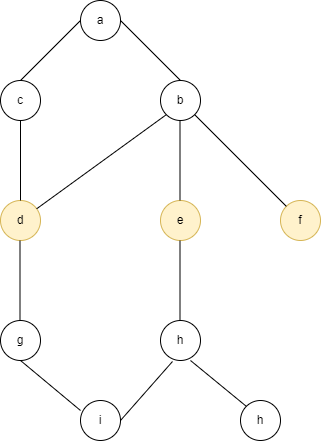
\includegraphics[scale=.5]{ant_catena.png}
    \caption{Evidenziata una anticatena}
\end{figure}

Le anticatene aggiungono ricchezza nella comprensione del dato ordinale poichè esprimono la nozione di $\textit{incomparabilità}$, propria 
dei dati non numerici. I dati di tipo ordinale presentano diverse sfaccetturare e sfumature che compongono il fenomeno in studio. Normalmente gran parte 
di questo tipo di informazione andrebbe persa con i classici approcci numerici, ma tramite gli insiemi parzialmente 
ordinati siamo in grado di costruire un oggetto formale non euclideo in grado di catturare alcune caratteristiche importanti 
dei nostri dati e di ricavarne dell'informazione, senza però trasformare e snaturare il dato dalla sua forma originaria con una conseguente
perdita di informazione.\\

\section{Estensioni lineari}

Un'estensione lineare è un ordinamento completo che contiene tutte le comparabilità del poset di input.  
L'idea è quella di trasformare alcune incomparabilità in comparabilità, in modo tale da ottenere un ordinamento completo che contiene tutte 
le comparabilità del poset di partenza. Per ottenere questo risultato si aggiunge comparabilità al poset finchè non si ottiene un ordinamento parzialmente
ordinato che non
può più essere esteso perchè è diventato lineare. \\
Gli oggetti che si creano da questo processo prendono il nome di $\textit{estensioni lineari}$. $\textit{Estensioni}$ poichè aggiungendo comparabilità
si estende l'insieme delle coppie comparabili del poset, $\textit{lineari}$ perchè non vi sono più incomparabilità. \\
Sia $P_1$ = (\{a, b, c, d, e\}, $\leq$) un poset, l'insieme delle sue estensioni lineari sono rappresentate in Figura 2.5 insieme 
al poset stesso. 
\begin{figure}[H]
    \centering
    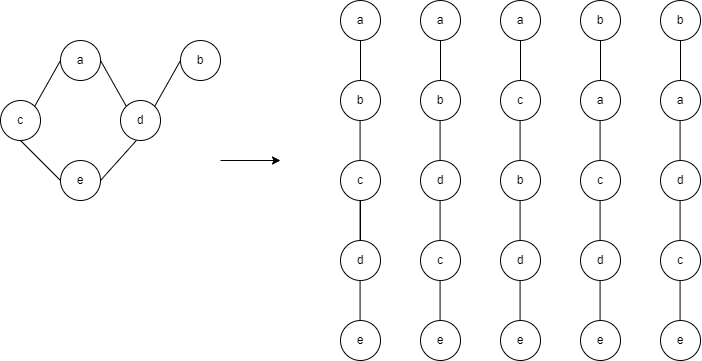
\includegraphics[scale=.5]{estensione_lin.png}
    \caption{Tutte le sole ed uniche estensioni lineari del poset $P_1$}
\end{figure}

Le estensioni lineari permettono di ricostruire univocamente il poset di partenza, difatti le comparabilità del poset sono tutte e solo le 
comparabilità comuni al suo insieme di estensioni lineari. Nell'esempio sopraillustrato possiamo vedere come l'elemento \say{e}, il quale è un minimo, si trovi
sempre all'ultimo posto in tutte e cinque le differenti estensioni lineari, mentre gli elementi \say{a} e \say{b}, i quali sono entrambi due
massimali, siano sempre al primo posto nelle diverse estensioni lineari. L'elemento \say{a} domina più elementi di quanti non ne domini 
\say{b}, intuitivamente quindi anche se \say{a} e \say{b} non sono comparabili si sviluppa il concetto che \say{a} \say{è maggiore} in qualche modo
di \say{b}. Questa intuizione si riproduce nell'estensione lineare nel fatto che \say{a} è più spesso al primo posto rispetto all'elemento \say{b}. \\
Di fatto possiamo osservare come queste catene sono ottenute ordinando, in tutti i diversi possibili modi, le coppie incomparabili del poset
di partenza, senza però andare a modificare le comparabilità già esistenti.
Perciò possiamo affermare che un poset è equivalente alle sue estensioni
lineari, ed attraverso di esse siamo in grado di trasformare un problema descritto da una struttura complessa a più dimensioni in una
struttura unidimensionale più semplice. \\
In termini pratici ciò che si ottiene è che l'analisi statistica su un ordinamento parzialmente ordinato può, nella maggior parte dei casi,
essere ricondotta all'analisi delle sue estensioni lineari, proprio grazie al fatto che queste individuano univocamente un poset. Come conseguenza, non si 
lavora più con degli oggetti multidimensionali, ma con degli ordinamenti completi semplici, i quali sono ricondicibili a variabili ordinali
multidimensionali. \\
\\
\\
Fin ora abbiamo introdotto il concetto di ordinamento parzialmente ordinato e le principali problematiche legate all'analisi di insiemi
di indicatori ordinali. I diagrammi di Hasse e le estensioni lineari sono differenti espressioni di un poset, che rappresentano e mantengono le 
fondamentali nozioni di comparabilità,  e di conseguenza di incomparabilità, che rendono i poset così particolari e non banali da analizzare e 
comprendere, sopratutto da un punto di vista matematico-statistico. Tuttavia questi elementi non bastano per avere una profonda comprensione
dell'argomento e
per effettuare una attenta analisi dei fenomeni qualitativi. Per questi motivi, sempre nell'ambito della teoria degli insiemi di cui fanno 
parte gli insiemi parzialmente ordinati, vi sono altri elementi che permettono, sempre mantenendo le nozioni di comparabilità ed incomparabilità,
di studiare e modelizzare il problema da una prospettiva matematica. \\
A differenza dei canonici metodi utilizzati per l'analisi di dati ordinali discussi precedentemente, le tecniche esposte di seguito hanno 
la peculiarità e la caratteristica di conservare l'ordine naturale dei dati ordinali. \\

\section{Rappresentazione matriciale di un insieme parzialmente ordinato}

Gli insiemi parzialmente ordinati possono essere rappresentati anche sotto forma matriciale, tramite le matrice Z di $\textit{dominanza}$
e la matrice G di $\textit{copertura}$. Di seguito vengono proposte le matrici G e Z per il poset $P_1$ rappresentato in Figura 2.5. 
\begin{align}
    Z = 
    \left( \begin{array}{ccccc} 1 & 0 & 1 & 1 & 1 \\
        0 & 1 & 0 & 1 & 0\\
        1 & 0 & 1 & 0 & 1\\
        1 & 1 & 0 & 1 & 1\\
        1 & 0 & 1 & 1 & 1 \end{array} \right)
    \mbox{                  }
    G = 
    \left( \begin{array}{ccccc} 0 & 0 & 1 & 1 & 0 \\
        0 & 0 & 0 & 1 & 0\\
        1 & 0 & 0 & 0 & 1\\
        1 & 1 & 0 & 0 & 1\\
        0 & 0 & 1 & 1 & 0 \end{array} \right)
\end{align}
\\
Le colonne e le righe di ambe due le matrici rappresentano gli elementi del poset $P_1$ = (\{a, b, c, d, e\}, $\leq$) \\
La matrice di copertura G rappresenta lo scheletro della relazione d'ordine; presenta degli \say{1} se un elemento copre un 
altro e \say{0} altrimenti. Mentre la matrice di dominanza Z esprime la relazione d'ordine in senso vero e proprio, l'\say{1}
è presente se e solo se un elemento domina un altro e \say{0} altrimenti. Per definizione ogni elemento domina se stesso, 
perciò la matrice Z presenta tutti \say{1} sulla diagonale principale. \\
Nell'esempio soprariportato l'elemento $Z_{1,3}$ è uguale ad 1 perchè \say{a} domina \say{c}, e per transitività \say{a} domina
\say{e}, perciò l'elemento di $Z_{1,5}$, che rappresenta la coppia \say{a}-\say{e}, è sempre pari ad 1. 
Nella matrice G invece, dato che vengono riportate solo le relazioni di copertura l'elemento di $G_{1,3}$ è sempre pari ad 1, 
dato che \say{a} copre \say{c}, ma a differenza della relazione di dominanza, la relazione di copertura non è transitiva, 
perciò \say{a} non copre \say{e}, da cui l'elemento $G_{1,5}$ è pari a 0. \\
\\
Un'ulteriore rappresentazione matriciale dei poset si ha tramite la matrice di \linebreak $\textit{mutual ranking probabilities}$
(MRP), la quale 
rappresenta al suo interno la quota di estensioni lineari in cui un elemento domina un'altro. Infatti i valori all'interno della MRP si ottengono tenendo conto di quante volte l'elemento i-esimo 
domina l'elemento j-esimo, pertanto
questa matrice esprime quanto intensamente i punti si dominano a vicenda. Inoltre si nota anche come la matrice 
MRP identifica univocamente il poset in quanto \say{contiene} al proprio interno la matrice di dominanza 
Z. Di seguito vi è la rappresentazione della matrice M di mutual ranking probabilities
del poset $P_{1}$. 
\begin{align}
    M = 
    \left( \begin{array}{ccccc} 1 & 0,4 & 0 & 0 & 0 \\
        0,6 & 1 & 0,2 & 0 & 0\\
        1 & 0,8 & 1 & 0,4 & 0\\
        1 & 1 & 0,6 & 1 & 0\\
        1 & 1 & 1 & 1 & 1 \end{array} \right)
    \mbox{                  }
\end{align}
\\
Il valore di $M_{1,2}$ indica che nel 40\% delle volte l'elemento \say{b} domina \say{a}, allo stesso 
modo $M_{2,1}$ pari a 0,60 indica che nel 60\% delle volte \say{a} domina \say{b}. L'elemento \say{e}, è 
un minimo in quanto viene sempre dominato da tutti gli altri elementi, di conseguenza la quinta ed ultima riga della matrice 
presentano tutti valori unitari. Come nella matrice di dominanza Z anche nella matrice M ogni elemento
domina se stesso, perciò la diagonale principale presenta tutti gli elementi pari ad 1. 
In questo modo i valori all'interno della matriche di mutual ranking probabilities rappresentano proprio la quota 
di estensioni lineari che classificano l'elemento i-esimo sopra l'elemento j-esimo. 
La matrice di MRP risulta di fondamentale importanza perchè da essa si estrae successivamente l'informazione
necessaria per creare il ranking finale. L'idea alla base è che dato che ogni colonna esprime quanto 
quell'elemento domina gli altri, di conseguenza la media della colonna indicherà quanto un punto tende ad essere 
dominante rispetto a tutti gli altri punti e questo si presenta come un primo approccio alla costruzione di un ranking
finale. Il raking è una struttura unidimensionale perciò per ottenerlo si richiede di effetturare una 
riduzione della dimensionalità della matrice di MRP n$\times$k. Vi sono differenti tecniche che 
effettuano la riduzione della dimensionalità, ma la più utilizzata è la Singular Value Decomposition(SVD). 

\section{Singular Value Decomposition}


La $\textit{Singular Value Decomposition}$(SVD) è ritenuta la soluzione ottimale a qualunque problema di approssimazione
dei dati di input[4]. All'interno della teoria degli insiemi parzialmente ordinati è utilizzata per effettuare
un'ottimale riduzione della dimensionalità sulla matrice di mutual ranking probabilities. L'idea alla base 
è che una matrice X, complessa o reale di dimensione m$\times$n si possa scrivere come il prodotto
di tre matrici; U, D, V. 
\begin{align}
    X = UDV^t
\end{align}
dove; \\
\\
$\bullet$ U è una matrice n$\times$k le cui colonne sono ortonormali.\\
\\
$\bullet$ D è una matrice diagonale k$\times$k i cui elementi sulla diagonale sono i valori singolari della matrice X 
in ordine descrescente. \\
\\
$\bullet$ V è una matrice ortogonale k$\times$k le cui righe e colonne sono ortonormali. \\
\\
\\
Vi è una duplice interpretazione del risultato della decomposione a valori singolari. \\
In un primo caso possiamo effettuare la seguente assimilazione: 
\begin{align}
    X = UDV^t = AV^t
\end{align}
Con A = UD.\\
In questo caso ogni profilo della matrice X viene ricostruito come somma pesata delle righe 
ortonormali di $V^t$, con pesi nelle righe di A. Di conseguenza le righe di A appaiono come le coordinate 
delle righe della matrice X sulla base formata dalle righe ortornormali di $V^t$, ciò significa che 
esse contengono l'informazione necessaria a ricostruire le righe di X, una volta scelta la base di riferimento
data dalle righe di $V^t$. \\
Nel secondo caso possiamo vedere la decomposione a valori singolari nel seguente modo; 
\begin{align}
    X = UDV^t = UQ
\end{align}
Con Q = D$V^t$. \\
Così facendo la base vettoriale è data dalle righe di Q e le righe di U sono i coefficienti
della combinazione lineare che trovano le righe di X. Bisogna però porre attenzione al fatto che le 
righe di Q sono date dalle righe di $V^t$ moltiplicate per i valori singolari, perciò non sono più 
normalizzate. Questo non pone di per sè dei problemi, si tratta semplicemente di una scelta da compiere 
durante l'analisi. \\

Possiamo quindi affermare che tramite la decomposizione a valori singolari(2.3) noi identifichiamo le 
coordinate UD che costruiscono la matrice X sulla base formata dalle righe ortonormali di $V^t$, come 
risultato si ha che conoscere UD equivale a conoscere la matrice originale X. \\
\\
La SVD è definita come la $\textit{soluzione ottimale}$ a qualunque problema di approssimazione dei dati 
di input, ma cosa garantisce questa ottimalità della decomposizione a valori singolari rispetto ad altre 
tecniche di riduzione della dimensionalità? \\
La risposta si trova nel Teorema di Eckart-Young il quale stabilisce 
come costruire la matrice $\hat{X}$ che meglio approssima la matrice di input X nella 
norma di Frobenius$\footnote[2]{La norma di Frobenius $\Vert{M}_{F}$ $\Vert$ di una matrice M n$\times$k è definita come $\Vert{M}_{F}$ $\Vert$ = $\sqrt{Tr(M^tM)}$}$. Di seguito viene enunciato il teorema di Eckart-Young;\\
\\
Sia X una matrice n$\times$k di rango k$\leq$ n, sia 0 < p $\leq$ k un intero fissato e sia X = UD$V^t$ la 
decomposzione a valori singolari di X. Indichiamo con $U_{[p]}$ la matrice n$\times$p composta 
dalle prime p colonne di U, con $V_{[p]}$ la matrice k$\times$p composta dalle prime p colonne di V e con 
$D_{[p]}$ la matrice p$\times$p composta dalle prime p righe e prime p colonne di D. La matrice 
\begin{align}
    \hat{X} = U_{[p]}D_{[p]}V_{[p]}^t = \sum_{i = 1}^{p} \sigma_{i} Z_{i}
\end{align}
minimizza la distanza $\Vert{X - \hat{X}}$ $\Vert_{F}$ nell'insieme delle matrici n$\times$k, di rango p.\\ 
Con questa scrittura il Teorema di Eckart-Young ci permette di vedere la decomposizione a valori singolari come la sovrapposizione di p
layers(strati) tutti con rango unitario, pesati per i valori singolari $\sigma_{i}$. \\
\\
La SVD effettua la riduzione della dimensionalità ponendo a zero i valori oltre i p-esimo nella matrice D, ciò significa che i valori da p+1
a k sono tutti nulli, di conseguenza restano solo k-p valori singolari non nulli. Ponendo a zero i valori singalori sulla matrice D vengono anche 
\say{annullati} i k-p valori delle colonne di U e righe di $V^t$. Di conseguenza la matrice $\hat{X}_{nxk}$ ha k colonne ma è di rango p. 
Come risultato ottengo che le righe della matrice approssimante $\hat{X}$ sono k dimensionali ma scrivibili come combinazione lineare di p vettori
linearmente indipendenti. \\
\\
La SVD è unica se i valori singolari della matrice A sono positivi, non crescenti e non degeneri, inoltre la decomposizione a valori singolari
è resistente alle permutazioni delle colonne di U e di V. Nella pratica perciò la SVD è unica, perchè anche se si scelgono diverse basi vettoriali
e diversi coefficienti lineari ciò che si ottiene è solo una diversa interpretazione della stessa matrice di input X. 

\section{Sistemi di indicatori multidimensionali}

All'atto pratico ciò che accade è che si devono gestire dei sistemi di indicatori multidimensionali(SMI), i quali si presentano come un insieme di k variabili 
congiuntamente rilevate su una data popolazione. Ad ogni unità statistica viene attribuito un punteggio, o in grado, su ogni 
variabile ed infine questi valori si presentano come una configurazione di punteggi sulle k variabili in studio. \\
Lo scenario sopra descritto è assai comune, se si pensa che una qualsiasi indagine statistica non si limita a raccogliere informazioni per una 
determinata variabile, ma cerca di recuperare quanta più informazione possibile e come risultato ci si ritrova con diverse centinaia di 
punteggi(profili) per ogni unità statistica. \\
La complessità, in questo tipo di analisi, è quella di tentare di costruire un qualche tipo di ordinamento, in modo tale da poter creare un unico  $\textit{ranking}$, 
ossia un ordinamento unidimensionale di facile e immediata comprensione. Quest'ordinamento però deve avere la fondamentale proprietà di 
preservare l'ordine dei profili, questo significa che se un profilo domina un altro nello SMI voglio che questa dominanza venga
mantenuta anche nel ranking finale. Ciò che stiamo cercando quindi è una mappa che effettua la riduzione della dimensionalità da un insieme di 
indicatori multidimensioni ad un ranking che preservi l'ordine in maniera stretta. \\
\\
Siano $V_{1}$, $V_{2}$, $V_{3}$, $V_{4}$, $V_{5}$ cinque variabili ordinali valutate su k = 5 scale con un numero di gradi $g_{i}$, ..., $g_{j}$ con j = 4, 
rilevate su $u_{1}$,...., $u_{7}$ unità statistiche. Alla generica unità statistica $u_{i}$ corrisponde un profilo di punteggi ordinali 
$p_{i}$ = ($u_{i1}$, $u_{i2}$, ..., $u_{i7}$) costituito dai diversi gradi che l'i-esima unità statistica assume sulle k variabili(Tabella 2.1). \\
\begin{table}[h!]
    \centering
    \begin{tabular}{||c c c c c c||} 
     \hline
           & $V_{1}$ & $V_{2}$ & $V_{3}$ & $V_{4}$ & $V_{5}$ \\ [0.5ex] 
     \hline\hline
     $u_{1}$ & 1 & 4 & 2 & 3 & 1 \\ 
     $u_{2}$ & 1 & 1 & 2 & 4 & 2 \\
     $u_{3}$ & 4 & 4 & 1 & 3 & 3  \\
     $u_{4}$ & 3 & 2 & 3 & 3 & 1  \\
     $u_{5}$ & 1 & 4 & 3 & 3 & 1  \\ 
     $u_{6}$ & 1 & 1 & 2 & 4 & 3 \\
     $u_{7}$ & 2 & 3 & 3 & 2 & 2 \\ [1ex] 
     \hline
    \end{tabular}
    \caption{Struttura di un sistema multidimensionale di indicatori ordinali}
    \label{table:1}
\end{table}

Il nostro obiettivo è costruire un ordinamento basato sui confronti tra diversi profili, ma per poterlo effettuare si rende necessario introdurre 
la nozione di ordinamento prodotto. \\
\\
L'ordinamento prodotto è un criterio d'ordine per, appunto, ordinare diversi profili. Dati due profili $p_{i}$ e $p_{j}$ con j $\neq$ i, si 
dice che il profilo $p_{j}$ domina il profilo $p_{i}$, se e solo se, i gradi di $p_{j}$ sono tutti non inferiori a quelli di $p_{i}$ e almeno
uno è superiore, in tal caso scriveremo $p_{i}$ $\blacktriangleleft $ $p_{j}$. \\
Se l'unità $u_{i}$ presenta punteggi più elevati o non inferiori a $u_{j}$ su tutte le variabili, allora $u_{i}$ avrà 
un punteggio maggiore rispetto a $u_{j}$. Utilizzando questo criterio è lampante il fatto che non è 
possibile ordinare in moto totale le diverse unità statistiche, a causa di punteggi \say{in conflitto}, ossia
nel caso in cui un'unità abbia punteggi maggiori su alcune variabili ma minori su altre. Ma alcuni 
confronti tra unità sono tuttavia possibili, permettendo di ottenere un ordinamento parzialmente ordinato 
su sistemi di indicatori multidimensionali.\\
\\
Lo scopo è quello di creare un ranking unidimensionale a partire da confronti multidimensionali fra unità
statistiche, per ottenere questo risultato ad ogni profilo si attribuisce un punteggio e successivamente
si ordinano questi punteggi in ordine decrescente creando così una classifica. Il punteggio attribuito ad ogni profilo esprime quanto 
quel profilo tende a dominare gli altri, creando così una nozione di \say{somiglianza} in base al punteggio ottenuto. Di conseguenza, 
in base alla distribuzione dei punteggi è possibile anche identificare cluster o pattern di profili, oltre che ad ottenere una classifica 
finale. \\
\\
Di seguito viene presentata la procedura utilizzata per ottenere il ranking[5]; \\
\\
1. Si crea l'insieme $\pi$ che contiene tutti i possibili profili originati dai punteggi degli attributi presenti nel sistema di 
indicatori multidimensionali. La cardinalità di $\pi$ è pari a $\vert$$\pi$$\vert$  = $g_{1}$$\cdot$$g_{2}$...$\cdot$$g_{j}$\\
2. Utilizzando il criterio dell'ordinamento prodotto si struttura in un insieme parzialmente ordinato $\pi$, il quale rappresenta lo 
\say{spazio} in cui collocare il calcolo dei punteggi dei profili. Lo spazio $\pi$ generalmente conterrà al suo interno sia i profili
osservati nel dataset che quelli non osservati. I profili non osservati hanno un valore prezioso, perchè aiutano a definire i 
gradi di dominanza anche fra i profili osservati. \\
3. Successivamente si costruisce l'insieme $\Omega$($\pi$) di tutte le possibili estensioni lineari di $\pi$. L'insieme $\Omega$($\pi$)
rappresenta l'insieme di tutti i possibili ordinamenti lineari di elementi che appartengo a $\pi$ che non violino le sue comparabilità.\\
4. Per ogni coppia di profili $p_{i}$ e $p_{j}$ appartenenti a $\pi$, si calcola la matrice di MRP, la quale al suo interno contiene
la frazione $P_{ij}$ di estensioni lineari nelle quali $p_{j}$ domina $p_{i}$. \\
5. Dopodichè si effettua la decomposizione a valori singalori della matrice P, P = UD$V^t$ e si estrae la prima colonna 
v = $(\mathbf{v_{i}, ..., v_{k}})^{t}$ della matrice V, i cui elementi rappresentano il grado di dominanza di ciascun profilo sugli altri.\\
6. Infine, ordinando i vari profili in ordine decrescente si ottiene la classifica finale. \\
\\
Questa procedura descrive il processo di creazione di un ranking unidimensionale a partire da un sistema di indicatori multidimensionali, nella prossima sezione
invece discuterò del concetto, estremamente importante, di incomparabilità.  
\\

\newpage

\section{Incomparabilità}

La trasformazione dei dati che avviene passando da un Insieme Parzialmente Ordinato ad un unico ranking unidimensionale comporta, ovviamente, una forzatura 
dei dati originali, oltre che una perdita di informazioni, questo perchè, come già spiegato nelle sezioni precedenti, le incomparabilità tra i diversi profili
vengono eliminate, ma ai fini di cercare di tenere conto di questa perdita di informazione è possibile calcolare un punteggio di incomparabilità per ogni profilo. 
Questo 
punteggio esprime non solo quanto stiamo distorcendo i dati originali nel posizionare un generico profilo nella posizione i-esima, ma ci fornisce anche un'idea 
dell'incertezza con cui leggere i valori nella classifica. Bisogna sempre ricordare, infatti, come i punteggi siano sempre ottenuti da indicatori multidimensionali 
e il valore 
che vediamo nella classifica è solo una sintesi; per esempio due profili, potrebbero anche essere poco confrontabili sul piano logico, perchè si trovano in 
situazioni molto 
diverse sul piano multidimensionale ed il punteggio di incomparabilità tiene conto proprio di questo. Se il punteggio di incomparabilità è alto significa che un 
profilo è stato molto distorto, inoltre il valore che ha ottenuto nel ranking è "meno sensato" rispetto a quegli elementi che hanno ottenuto un valore basso di 
incomparabilità.
A causa della grande rilevanza logica che il punteggio di 
incomparabilità ha, è spesso consigliato calcolarlo, ma sopratutto di tenerne conto quando si legge la classifica finale. 
\\
\\
Per calcolare il punteggio di incomparabilità si parte dalla matrice di Mutual Raking Probabilities e si costruisce un'ulteriore matrice, chiamata 
LIM(\textit{Lexicographic Incomparability Matrix}), ossia Matrice di Incomparabilità Lessicografica. \\
I valori all'interno di quest'ultima matrice si ricavano prendendo per ogni coppia riga-colonna \textit{ij} e per ogni coppia colonna-riga \textit{ji} della 
matrice di MRP il valore minimo e lo si pone nella posizione \textit{ij} e \textit{ji} della matrice LIM. Formalmente; $LIM_{ij}$ $\leq$ \textit{min}($MRP_{ij}$, $MRP_{ji}$).
La matrice LIM, perciò risulta essere una matrice simmetrica e per definizione presenta tutti valori nulli sulla diagonale. Nel seguente esempio si propone la 
matrice LIM ricavata dalla matrice di MRP in 2.2.\\

\begin{align}
    LIM = 
    \left( \begin{array}{ccccc} 0 & 0,4 & 0 & 0 & 0 \\
        0,4 & 0 & 0,2 & 0 & 0\\
        0 & 0,2 & 0 & 0,4 & 0\\
        0 & 0 & 0,4 & 0 & 0\\
        0 & 0 & 0 & 0 & 0 \end{array} \right)
    \mbox{                  }
\end{align}

Come si può notare la matrice è simmetrica e presenta valori nulli sulla diagonale. L'elemento $LIM_{2,1}$ coindice con $LIM_{1,2}$ ed è pari a 0,4, questo perchè
nella matrice di MRP M presentata al punto 2.2, il valore di $M_{2,1}$ è pari a 0,60, mentre $M_{1,2}$ è pari a 0,40, di conseguenza dato che per costruire
la matrice LIM prendiamo il più piccolo dei due valori e la matrice è simmetrica, gli elementi $LIM_{2,1}$ e $LIM_{1,2}$ sono uguali e pari a 0,40. Con il medesimo
criterio vengono calcolati gli altri elementi della matrice LIM. \\
Una volta ottenuta la matrice LIM, si prosegue poi ad effettuare una riduzione della dimensionalità, per lo scopo di queste analisi è sempre stata utilizzata la SVD, 
per poi ottenere come risultato finale un punteggio di incomparabilità. \\
\\
In questo capitolo ho descritto le principali nozioni teoriche della teoria degli ordinamenti parziali, nel prossimo capitolo descriverò le mie analisi statistiche. 
\newpage

\chapter{Analisi}

Lo scopo della mia analisi è quello di sviluppare il concetto di \say{competitività} tra diversi stati a partire dal dataset del
European Innovation Scoreboard(EIS) dell'Unione Europea; i dati dell'EIS vengono raccolti e rilasciati ogni anno ed hanno lo scopo di 
valutare le performance dei vari stati europei sotto diversi aspetti. \\
Utilizzando gli indicatori presenti nel dataset si è cercato di costruire il concetto di \say{competitività} scomponendolo nelle sue dimensioni caratterizzanti, successivamente dopo aver calcolato una classifica degli stati più competitivi per ogni dimensione, verrà anche calcolato un punteggio di \say{incomparabilità} per ogni stato, il quale ha
il duplice scopo di fornire informazioni su quanto sia distorto il valore ottenuto nella classifica e di permettere una più chiara interpretazione ed un più 
cristallino confronto tra gli stati, come già spiegato nel secondo capitolo di questa tesi. \\
\\
Per le analisi è stato utilizzato il software open source R, version 4.1.1 (2021-08-10). In particolare sono state utilizzate le librerie \texttt{dplyr}, \texttt{funModeling}, 
\texttt{parsec} e \texttt{netrankr}. \\
La libreria \texttt{dplyr} è stata creata da Hadley Wickham$\footnote[3]{Hadley Alexander Wickham è uno statistico neozelandese direttore scientifico di RStudio 
Inc. e professore aggiunto in diversi atenei, tra cui la Standford University[6].}$ e Romain Francois$\footnote[4]{Romain Fracois lavora attivamente nella R community 
ed è l'autore e cooperatore di diverse altre librerie su R come Rcpp e plyr[7]}$  con lo scopo di fornire una serie di strumenti molto ampi per lavorare e manipolare 
dataframe, la libreria \texttt{funModeling} è una delle librerie più utilizzate per analisi esplorative e la preparazione dei dati alle analisi creata da 
Pablo Casas$\footnote[5]{Pablo Casas è data scientist e professore di AI all'Università di Buenos Aires[8].}$, mentre la libreria \texttt{parsec} comprende strumenti per 
l'analisi degli Insiemi Parzialmente Ordinati, con una particolare attenzione ai sistemi di indicatori multidimensionali, realizzata da Alberto Arcagni $\footnote[6]{Alberto 
Arcagni è prefessore associato di statistica all'Università Sapienza di Roma[9].}$. Infine, la libreria \texttt{netrankr} che permette di utilizzare metodi legati
all'analisi di ranking parziali nelle reti, è stata ideata da David Schoch$\footnote[7]{David Schoch è uno studente post-doc all'Università di Konstanza in Germania[10].}$. 
\\

\newpage

\section{Descrizione dei dati}

Sono stati scaricati i dati dell'EIS, dal 2014 al 2021, dal sito dell'Unione Europea$\footnote[8]{\url{https://ec.europa.eu/research-and-innovation/en/statistics/performance-indicators/european-innovation-scoreboard/eis}}$[11]. I dati dell'EIS vengono raccolti e pubblicati dal 2001 e, 
durante il corso degli anni gli indicatori utilizzati hanno subito delle variazioni. Queste modifiche sono state effettuate per migliorare
attivamente la qualità delle analisi ed assicurarsi che i risultati riflettano i cambiamenti economici, politici, demografici e sociali degli stati. \\
\\
Il dataset si presenta composto da otto variabili e 71514 osservazioni. 
La variabile \texttt{Perf} esprime il voto finale ottenuto da ciascuno stato nei diversi indicatori; ha quattro possibili valori \say{Leader}, \say{Strong}, 
\say{Moderate} e \say{Emerging}. \say{Leader} viene assegnato a tutti quei paesi che hanno ottenuto una performance relativa maggiore del 125\% rispetto alla media
europea. \say{Strong} viene, invece, assegnato ai paesi che hanno avuto una performance relativa tra il 100 \% ed il 125 \% rispetto alla media europea. Mentre 
\say{Moderate} viene applicato a tutti quegli stati che hanno ottenuto una performance tra il 70\% ed il 100\%, sempre rispetto alla media europea. Infine 
\say{Emerging} viene assegnato ai paesi che hanno ottenuto una performance al di sotto del 70\% rispetto alla media 
europea$\footnote[9]{\url{https://www.eustat.eus/elementos/European-Innovation-Scoreboard-2021-Methodology-Report/inf0019111_c.pdf}}$[12]. \\
La variabile \texttt{Year} assume tutti i valori dal 2014 al 2021, ed appunto, indica l'anno a cui si riferisce ogni indicatore. \\
\\
Vi sono quattro diverse variabili che forniscono indicazioni geografiche, esse sono le variabili \texttt{Country}, \texttt{CountryName}, \texttt{Region} e \texttt{Zone}. Le variabili \texttt{Country} e \texttt{Region} riportano la stessa informazione, ossia il nome del paese in formato 
ISO 3166-1 aplha 2$\footnote[10]{ISO 3166-1 alpha 2 è un sistema di codificazione dei paesi del mondo a due cifre.}$, mentre \texttt{CountryName} invece indica il nome 
del paese in inglese. La variabile \texttt{Zone} indica se il paese appartiene o meno all'Unione Europea, infatti oltre i ventisette paesi che compongono 
l'Unione Europea(Austria, Belgio, Bulgaria, Cipro, Croazia, Danimarca, Estonia, Finlandia, Francia, Germania, Grecia, Irlanda, Italia, Lettonia, Lituania, Lussemburgo,
Malta, Paesi Bassi, Polonia, Portogallo, Repubblica Ceca, Romania, Slovacchia, Slovenia, Spagna, Svezia, Ungheria) sono presenti anche undici paesi che non ne fanno
parte, questi sono: Islanda, Israele, Norvegia, Regno Unito, Bosnia ed Erzegovina, Montenegro, Nord Macedonia, Serbia, Svizzera, Turchia ed 
Ucraina. 
Data la rindondanza di informazione di tipo geografico si è provveduto a tenere in analisi solo la variabile \texttt{CountryName}.
\\
Infine la variabile \texttt{Indicator} ha come possibili valori i settantasei diversi indicatori presenti nel dataset, questo perchè in forma originaria gli indicatori 
raccolti non sono stati presentati come variabili, quindi come colonne, ma come osservazioni, quindi come righe. Ai fini di consetire una migliore comprensione 
dei dati e per agevolare le analisi, i dati sono stati posti nel classico formato \say{indicatori $\times$ per unità statistiche} dove le colonne sono gli indicatori 
e le righe i diversi stati. \\
\\
Infine la variabile \texttt{Value} esprime, per ogni indicatore il suo valore numerico. Può assumere sia valori positivi che negativi ed ha un minimo pari a -19,862
ed un massimo pari a 1620,017
\\
\\
Di seguito viene riportata una tabella dove vengono evidenziate le principali informazioni per ogni variabile qualitativa; \\

\begin{table}[h!]
    \centering
    \begin{tabularx}{0.8\textwidth} { 
        | >{\raggedright\arraybackslash}X 
        | >{\centering\arraybackslash}X 
        | >{\raggedleft\arraybackslash}X | }
        \hline
        \textbf{Nome variabile} & \textbf{Tipo} & \textbf{Numero livelli} \\
        \hline
        \texttt{Indicator} & qualitativa & 76  \\
        \hline
        \texttt{Perf} & qualitativa & 4 \\
        \hline
        \texttt{Year} & qualitativa & 7 \\
        \hline
        \texttt{Zone} & qualitativa & 2 \\
        \hline
        \texttt{Country} & qualitativa & 38 \\
        \hline
        \texttt{CountryName} & qualitativa & 38 \\
        \hline
        \texttt{Region} & qualitativa &  279\\
        \hline
        \texttt{RegionName} & qualitativa & 279 \\
        \hline
    \end{tabularx}
    \caption{Tabella delle variabili}
    \label{table:1}
\end{table}

Solo l'1,89\% delle osservazioni presentano dati mancanti, perciò ai fini dell'analisi si è deciso di porre queste osservazioni pari a zero. 
Questo perchè l'eliminazione di queste righe
avrebbe portato ad una perdita di informazione, inoltre dato lo scarso numero di osservazioni che presentano questo problema, 
la sostituzione effettuata non 
avrà grandi ripercussioni sulle analisi. \\
\\
Come già accennato precedentemente la variabile \texttt{Indicator} presenta come valori i 76 indicatori che formano l'EIS, cosicché 
per agevolare le 
analisi si è proceduto a porre gli indicatori nella più usuale forma di colonna. \\
\\
Da un'attenta analisi ed osservazione emergono quattro grandi dimensioni in cui ricadono tutti gli indicatori utilizzati; Economia, Demografia, 
Istruzione ed Innovazione. \\
L'economia viene definita come \say{\textit{il sistema e l'organizzazione dei mercati, risorse, della produttività e del complesso di scambi, produzioni e commerci di beni e 
servizi, dei sistemi di finanziamenti, investimenti e di fondazione di attività economiche in ogni settore, di ogni dimensioni e ad ogni 
scopo$\footnote[11]{\url{https://it.wikipedia.org/wiki/Economia}}$}}[13]. In questa categoria perciò rientrano tutti quegli indicatori che hanno un legame, diretto o 
indiretto con il commercio, la circolazioni di beni, servizi e materie prime, oltre che i più conosciuti indicatori come il GDP(Gross Domestic Product). \\
La demografia invece viene definita come \say{\textit{lo studio quantitativo, fondato sull'indagine statistica, dei fenomeni concernenti la 
popolazione$\footnote[12]{Britannica Dictionary}$}}[14], appartegono a questa dimensione alcuni tra i più semplici indicatori demografici, come il tasso di crescita 
annuale della popolazione e la sua densità. \\
Nella dimensione dell'istruzione rientrano principalmente tutti quegli indicatori che misurano, direttamente o indirettamente, il grado di scolarità della 
popolazione di uno stato, ma fanno sempre parte di questa categoria anche gli indicatori che valutano quanto è attivo ed attrativo il sistema educativo nazionale. \\
L'innovazione è forse la dimensione più difficilmente definibile e inquadrabile, cionondimeno ho cercato di fornire, in modo molto intuitivo, una 
definizione che potesse aiutarmi a meglio definire questa categoria. In questa analisi la dimensione dell'innovazione è stata intesa come quei settori, all'interno
della politica e delle istituzioni di uno stato, che hanno lo scopo di migliorare servizi o beni esistenti, con una particolare attenzione  
alle tecnologie dell'informazione e alle tematiche ambientali. \\
\\
Di seguito vengono riportare quattro differenti tabelle che mostrano, per ogni dimensione, quali indicatori la compongono. \\
\\
\begin{table}[h!]
    \centering
    \begin{tabular}{ |l|l| }
        \hline
        \multicolumn{2}{|c|}{\textbf{Economia}} \\
        \hline
        2.1 & Finance and support\\
        \hline
        2.2 & Firm investments \\
        \hline
        4.1 & Employment impacts \\
        \hline
        4.2 & Sales impacts \\
        \hline
        5.2.1 & Enterprise births \\
        \hline
        5.4.1 & Ease of starting a business \\
        \hline
        2.1.2 & Venture capital expenditures \\
        \hline
        2.1.3 & Direct and indirect government support of business R\&D \\
        \hline
        2.2.1 & R\&D expenditure in the business sector \\
        \hline
        2.2.2 & Non-R\&D innovation expenditures\\
        \hline
        2.3.2 & Employed ICT specialists \\
        \hline
        4.3.1 & Resource productivity \\
        \hline
        5.1.2 & Average annual GDP growth \\
        \hline
        5.1.3 & Employment share Manufacturing \\
        \hline
        5.1.4 & Employment share High and Medium high-tech \\
        \hline
        5.1.5 & Employment share Services  \\
        \hline
        5.1.7 & Turnover share SMEs  \\
        \hline
        5.1.8 & Turnover share large enterprises  \\
        \hline
        5.1.9 & Foreign-controlled enterprises – share of value added \\
        \hline
        5.2.2 & Total Entrepreneurial Activity  \\
        \hline
        5.2.3 & FDI net inflows  \\
        \hline
        5.2.4 & Top R\&D spending enterprises  \\
        \hline
        5.4.2 & Basic-school entrepreneurial education and training  \\
        \hline
        5.2.5 & Buyer sophistication  \\
        \hline
        5.1.1 & GDP per capita (thousands)\\
        \hline
      \end{tabular}
      \caption{Tabella delle variabili che formano la dimensione dell'Economia}
    \label{table:1}
\end{table}

Come si può notare dai nomi delle variabili che compongono questa dimensione, siamo di fronte ad una variegato insieme di indicatori, 
i quali spaziano da ambiti prettamente economici, come la crescita annuale del prodotto interno lordo(5.1.2-Average annual GDP growth),
ad ambiti più complessi, che però hanno sempre un impatto sull'economia come, ad esempio l'impatto sulle vendite(4.2-Sales impacts). Esso, viene infatti definito 
come \textit{la misura dell'impatto economico delle innovazioni che include tre diversi indicatori; la misura dell'export di tecnologie medio-alte, l'export 
di servizi knowledge-intensive e le vendite dovute ad attività di innovazione$\footnote{\url{https://www.eustat.eus/elementos/European-Innovation-Scoreboard-2021-Methodology-Report/inf0019111_c.pdf}}$}, per questa e 
tutte le altre definizioni degli indicatori si rimanda al report sulla metodologia pubblicato sul sito dell'Unione Europea$\footnote{\url{https://www.eustat.eus/elementos/European-Innovation-Scoreboard-2021-Methodology-Report/inf0019111_c.pdf}}$[12]. 
Difatti in questa dimensione rientrano anche tutti quegli indicatori che hanno un impatto indiretto sull'economia, come ad esempio il numero di nuove 
imprese nate in un determinato periodo(5.2.1-Enterprise births), questo perchè le imprese possiedono un ruolo determinante all'interno del sistema economico 
capitalistico, in quanto producono beni e servizi. Per questi motivi è importante ed essenziale tenere in considerazione anche questi aspetti all'interno 
della dimensione economica. 
\\
\\
Successivamente vengono riportare in tabella le variabili che compongono la dimensione \say{Demografia}; \\

\begin{table}[h!]
    \centering
    \begin{tabular}{ |l|l| }
        \hline
        \multicolumn{2}{|c|}{\textbf{Demografia}} \\
        \hline
        5.6.1 & Population size \\
        \hline
        5.6.2 & Average annual population growth \\
        \hline
        5.6.3 & Population density \\
        \hline
        5.4.4 & Rule of law \\
        \hline
      \end{tabular}
      \caption{Tabella delle variabili che formano la dimensione della Demografia}
    \label{table:1}
\end{table}

La dimensione demografica è quella che contiene il minor numero di indicatori, questo perchè lo studio statistico della popolazione non era tra gli obiettivi 
della analisi per cui questi dati sono stati raccolti. Tuttavia, avere anche solo una minima parte di informazione demografica, sopratutto quando si fa un'analisi 
con lo scopo di comparare stati diversi tra di loro, è sempre utile, anche per avere una migliore e più completa comprensione dei risultati. Di questa dimensione
fanno parte indicatori strettamente legati alla misura della quantità della popolazione come la dimensione della popolazione(5.6.1-Population size), la 
crescita media annuale della popolazione(5.6.2-Average annual population growth) e la densità di popolazione(5.4.4-Rule of law). La norma di 
legge(5.4.4-Rule of law), invece esprime un concetto differente rispetto agli altri indicatori; si riferisce infatti, a quanto i cittadini abbiano fiducia 
nelle forze di polizia e nelle istituzioni di uno stato. Questa variabile è stata posta in questa dimensione perchè, seppur in un modo non tradizionale, esprime
dell'informazione sulla popolazione che compone uno stato. \\

\newpage 

Di seguito viene mostrata la tabella contenente gli indicatori che appartengono alla dimensione \say{Istruzione}; \\

\begin{table}[h!]
    \centering
    \begin{tabular}{ |l|l| }
        \hline
        \multicolumn{2}{|c|}{\textbf{Istruzione}} \\
        \hline
        1.1 & Human resources\\
        \hline
        1.2 & Attractive research systems \\
        \hline
        1.1.1 & New doctorate graduates \\
        \hline
        1.1.2 & Population with tertiary education \\
        \hline
        1.1.3 & Population involved in lifelong learning \\
        \hline
        1.2.1 & International scientific co-publications \\
        \hline
        1.2.2 & Scientific publications among the top 10\% most cited  \\
        \hline
        1.2.3 & Foreign doctorate students as a \% of all doctorate students \\
        \hline
        3.2.2 & Public-private co-publications \\
        \hline
      \end{tabular}
      \caption{Tabella delle variabili che formano la dimensione dell'Istruzione}
    \label{table:1}
\end{table}

La dimensione dell'istruzione contiene al suo interno tutti quegli indicatori che esprimono dell'informazione non solo sul sistema educativo di un paese, come 
la percentuale di popolazione che possiede un'educazione terziara(1.1.2-Population with tertiary education) ed il numero di nuovi dottori di
ricerca(1.1.1-New doctorate graduates), ma anche sull'attrattività del sistema di ricerca(1.2-Attractive research systems, 1.2.3-Foreign doctorate students as a \% of all doctorate students)
e la disponabilità di personale altamente qualificato(1.1-Human resources). L'istruzione risulta molto importante quando si parla di 
\say{competitività} di un paese; questo perchè, se uno stato è in grado non solo di formare delle persone istruite e competenti, ma anche di 
attrarre con il suo sistema scolatistico ed accademico studenti dall'estero esso si presenta come un paese \say{attraente} dal punto di vista
accademico e perciò competitivo nel campo.\\

\newpage

Succesivamente viene riportata la tabella con le variabili che compongono la dimensione \say{Innovazione};\\

\begin{table}[h!]
    \centering
    \begin{tabular}{ |l|l| }
        \hline
        \multicolumn{2}{|c|}{\textbf{Innovazione}} \\
        \hline
        1.3 & Digitalisation\\
        \hline
        2.3 & Use of information technologies \\
        \hline
        3.1 & Innovators\\
        \hline
        3.2 & Linkages \\
        \hline
        3.3 & Intellectual assets \\
        \hline
        4.3 & Environmental sustainability \\
        \hline
        5.3.1 & In-house product innovators with market novelties \\
        \hline
        1.3.2 & Individuals with above basic overall digital skills \\
        \hline
        2.3.1 & Enterprises providing ICT training \\
        \hline
        3.1.1 & SMEs introducing product innovations  \\
        \hline
        3.1.2 & SMEs introducing business process innovations \\
        \hline
        3.2.1 & Innovative SMEs collaborating with others  \\
        \hline
        4.1.1 & Employment in knowledge-intensive activities \\
        \hline
        3.2.2 & Public-private co-publications  \\
        \hline
        3.3.1 & PCT patent applications  \\
        \hline
        3.3.2 & Trademark applications  \\
        \hline
        3.3.3 & Design applications \\
        \hline
        4.2.1 & Exports of medium and high technology products\\
        \hline
        4.2.2 & Knowledge-intensive services exports\\
        \hline
        4.2.3 & Sales of new-to-market and new-to-firm innovations \\
        \hline
        5.3.2 & In-house product innovators without market novelties \\
        \hline
        5.3.3 & In-house business process innovators \\
        \hline
        5.3.4 & Innovators that do not develop innovations themselves \\
        \hline
        5.3.5 & Innovation active non-innovators \\
        \hline
        5.3.6 & Non-innovators with potential to innovate \\
        \hline
        5.3.7 & Non-innovators without disposition to innovate \\
        \hline
        5.4.3 & Government procurement of advanced technology products \\
        \hline
        5.5.2 & Greenhouse gas emissions intensity of energy consumption \\
        \hline
        5.5.3 & Eco-Innovation Index \\
        \hline
        4.3.3 & Environment-related technologies \\
        \hline
        5.5.2 & Greenhouse gas emissions intensity of energy consumption \\
        \hline
        4.3.2 & Air emissions by fine particulates  \\
        \hline
        5.5.1 & Circular material use rate \\
        \hline
        2.2.3 & Innovation expenditures per person employed \\
        \hline
        4.1.2 & Employment in innovative enterprises  \\
        \hline
        5.1.6 & Employment share Knowledge-intensive services \\
        \hline
        2.1.1 & R\&D expenditure in the public sector \\
        \hline
      \end{tabular}
      \caption{Tabella delle variabili che formano la dimensione dell'Innovazione}
    \label{table:1}
\end{table}

La dimensione dell'innovazione è la più numerosa tra le diverse dimensioni, inoltre sempre questa dimensione, come già accennato precedentemente, è stata anche la più 
complessa e meno lineare da definire e come conseguenza, il ventaglio di indicatori che la compongono è molto vario e differente. Al suo interno, 
infatti, spaziamo da indicatori prettamente incentrati sulla digitalizzazione(1.3-Digitalisation, 2.3.1-Enterprises providing ICT training), a indicatori incentrati
sulla sostenibilità ambientale(4.3-Environmental sustainability, 5.5.3-Eco-Innovation Index, 4.3.3-Environment-related technologies), passando infine ad indicatori 
sugli investimenti di enti pubblici e privati in ricerca e sviluppo(R\&D expenditure in the public sector). \\
\\
\\
In questa sezione sono stati presentati i dati ed è stata fatta una breve panoramica sugli indicatori che compongono il dataset, mentre 
nella prossima sezione si presenteranno
le tecniche di analisi utilizzate. 
\newpage

\section{Analisi statistiche}

Una volta individuate le quattro dimensioni che compongono il concetto di competitività, si è proceduto a creare quattro differenti dataset, uno per ogni dimensione, ciascuno dei quali contenente le variabili 
che lo compongono. Ogni dataset presenta osservazioni dal 2014 al 2021, ad eccezione per la dimensione \say{Demografia}, la quale presenta dati, per ogni indicatore, 
solo del 2021.\\
\\
Tramite le librerie \texttt{parsec} e \texttt{netrankr} si è calcolata la matrice M di Mutual Ranking Probabilities(MRP)per ogni dimensione, prima di fare questo
però, si è associato, per ogni dimensione, una riga all'anno e allo stato corrispondende 
tramite la funzione di R \texttt{rownames}. Così facendo, ogni punteggio ottenuto nel ranking finale è associato allo stato e all'anno corrispondente. Successivamente, 
per effettuare la riduzione della dimensionalità, si è applicata la Singular Value Decomposition(SVD) su ogni matrice M. Infine, ordinando in ordine decrescente 
il risultato unidimensionale ottenuto con la SVD, si è ottenuto come risultato il ranking finale. I grafici dei ranking sono stati 
creati utilizzando la funzione \texttt{plot} di R con l'asse delle ordinate che rappresenta i punteggi dei ranking e l'asse 
delle ascisse presenta un indice di numeri a partire dal valore nullo.  \\
\\
\\
Infine per creare i punteggi di incomparabilità si è calcolata la matrice di Incomparabilità 
Lessicografica(LIM)$\footnote[15]{Per la teoria sul calcolo della matrice di Incomparabilità Lessicografica si rimanda alla sezione 2.7 di questa tesi}$, 
per ogni dimensione. Per fare ciò si è 
utilizzato il seguente codice. \\

\begin{verbatim}
    LIM <- matrix(NA_real_, NCOL(M), NCOL(M))
        for (i in seq_len(NCOL(LIM)))
            for (j in seq_len(NCOL(LIM)))
                LIM[i,j] <- min(min(M[i,j], M[j, i])) 
\end{verbatim}

La prima riga crea la matrice di Incomparabilità Lessicografica(LIM) utilizzando le colonne della matrice di Mutual Ranking Probabilities M, con il primo \texttt{for} cicla su tutte le righe della 
matrice LIM, mentre il secondo \texttt{for} invece cicla su tutte le sue colonne. Infine l'ultima riga seleziona l'elemento minimo per ogni coppia di riga e colonna di M e li pone come il 
j-esimo e l'i-esimo elemento della matrice LIM. \\
Infine, si effettua la Singular Value Decomposition sulla matrice LIM e si ordina il risultato in modo da ottenere la classifica di incomparabilità tra paesi. 
Per ottenere i grafici dell'incomparabilità, si sono prima normalizzati i risultati ottenuti nel ranking tramite l'avarage 
height$\footnote[16]{L'avarage height di un elemento x appartenente ad un poset finito P è il numero di elementi attesi sotto ad x in un'estensione casuale di P[15]}$, dopodichè tramite la 
funzione \texttt{plot} di R, si sono creati i grafici con i punteggi di incomparabilità sull'asse delle ascisse e il rispettivo 
ranking sull'asse delle ordinate. 


\newpage

\chapter{Conclusioni}

In questo capitolo analizzerò i risultati raggiunti tramite le analisi illustrate nella sezione 3.2 del capitolo precedente. Queste conclusioni non voglio essere una 
descrizione precisa e puntuale riguardante la Demografia, l'Economia, l'Istruzione e l'Innovazione degli stati analizzati, ma sono invece da interpretare come uno spunto iniziale, per 
introdurre una riflessione sulle condizioni di questi settori nei diversi stati europei e non. Queste conclusioni non vogliono neanche essere un giudizio di alcun modo 
sui differenti paesi, ma sono solo l'interpretazione, alla luce di conoscenze personali e ricerche più approfondite, dei risultati ottenuti dall'analisi oggetto di studio 
di questa tesi.  \\
\\
Per ogni dimensione verranno prima presentati i risultati riguardanti il ranking e successivamente verranno discussi i risultati ottenuti tramite i punteggi di incomparabilità. 

\newpage

\section{Economia}


Per aiutare nella comprensione dei risultati viene riportato di seguito il grafico della distrubuzione della classifica della dimensione dell'Economia. 
\begin{figure}[H]
    \centering
    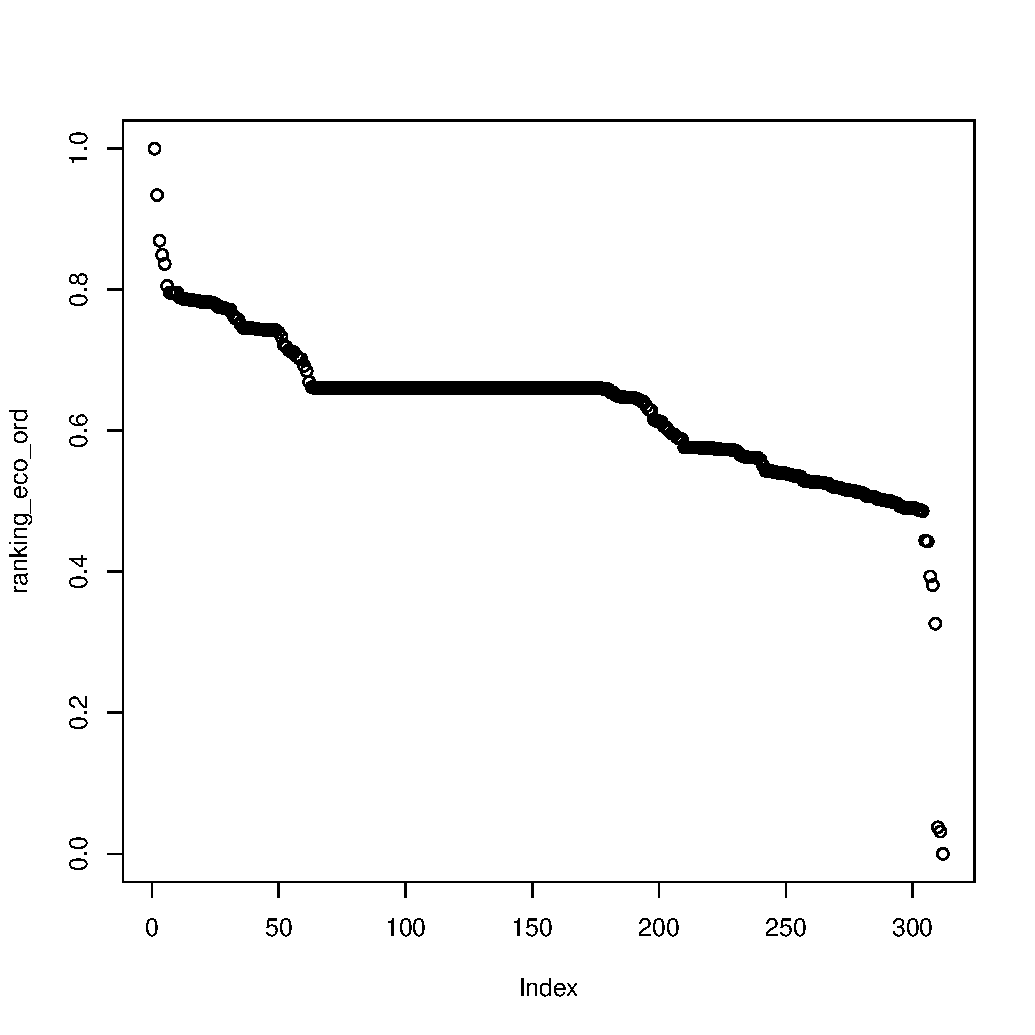
\includegraphics[scale=.5]{ranking_eco_norm.pdf}
    \caption{Grafico della classifica della dimensione dell'Economia}
\end{figure}

Il grafico rappresenta la classifica finale dei diversi paesi oggetto di analisi, dal 2014 al 2021. Sull'asse delle ordinate è presente il punteggio ottenuto da ogni stato
normalizzato in un intervallo [0-1],
mentre sull'asse delle ascisse è invece presente una sequenza di numeri che parte dal valore nullo. 
I punti sul grafico rappresentanto i trecentododici paesi presenti nella classifica; in questo ranking, infatti, sono presenti tutti e ventisette i paesi che compongono 
l'Unione Europea, a cui si aggiungono gli undici paesi elencati nella sezione 3.1. Infine ai trentotto paesi si aggiunge anche la media europea, calcolata ogni anno, per 
tutti gli otto anni presi in considerazione. In totale, perciò, vi sono trentanove osservazioni per ciascuno degli otto anni, le quali in totale fanno trecentododici 
osservazioni. \\
Come possiamo vedere dal grafico, sono solo cinque i paesi che raggiugnono un punteggio non inferiore a 0.80, con un valore massimo pari a 1,
mentre tutti gli altri paesi sono compresi tra un valore
di [0.80;0.50] Vi sono solo unicamente otto paesi con un valore inferiore a 0.50, con il valore più basso pari a 0.00. Inoltre, 
dalla distribuzione dei punti si può vedere come la maggior parte dei paesi assuma un valore pari a 0.66, al di sotto di questo valore vi è una tendenza discendente, 
fino ad un valore di 0.48, allo stesso modo oltre il valore di 0.66 i punti assumono sempre un valore maggiore, fino al valore di massimo di 1. \\
\\
Di seguito viene riportata la tabella che mostra tutti i punteggi normalizzati in un intervallo [0-1] ottenuti dai vari stati nei diversi anni; 
\newpage 

\setlength\tabcolsep{2pt}
\begin{longtable}[c]{|c|c|c|c|c|c|}
    \hline
    \textbf{Posizione} & \textbf{Paese} & \textbf{Punteggio} & \textbf{Posizione} & \textbf{Paese} & \textbf{Punteggio}\\
    \hline
    1° & UK-2020 & 1.0000 & 36° & Finland-2017 & 0.7433  \\ 
    \hline
    2°	& UK-2019 & 0.9342 & 36° & Finland-2018 & 0.7433 \\ 
    \hline
    3°	& UK-2017 & 0.8696 & 37° & Latvia-2014 & 0.7425 \\ 
    \hline
    4°	& UK-2018 & 0.8496 & 37° & Latvia-2015	& 0.7425 \\ 
    \hline
    5°	& UK-2021 & 0.8365 & 38° & Germany-2020 & 0.7394 \\ 
    \hline
    6°	& Norway-2020 & 0.8055 & 39° & Germany-2019 & 0.7336 \\ 
    \hline
    7°	& Portugal-2014	& 0.7958 & 40°	& Montenegro-2017 & 0.7217 \\ 
    \hline
    7°	& Ukraine-2014 & 0.7958  & 41°	& Montenegro-2020 & 0.7189 \\ 
    \hline
    7°	& Ukraine-2015 & 0.7958 & 42° & Norway-2014 & 0.7144 \\
    \hline
    7° & Ukraine-2016 & 0.7958 & 43° & Turkey-2015 & 0.7119 \\
    \hline
    8° & Turkey-2014 & 0.7889  & 44° & Cyprus-2016 & 0.7113 \\
    \hline
    9° & Israel-2014 & 0.7873 & 45° & Switzerland-2014 & 0.7061 \\
    \hline
    10° & Serbia-2014 & 0.7872 & 46° & Croatia-2014 & 0.7029 \\
    \hline
    11° & Montenegro-2019 & 0.7860 & 47° & Montenegro-2016 & 0.7015 \\
    \hline
    12° & Latvia-2017 & 0.7856 & 48° & Romania-2018 & 0.6922 \\
    \hline
    13° & France-2015 & 0.7855 & 49° & Croatia-2015 & 0.6847 \\
    \hline
    14° & Croatia-2018	& 0.7847 & 50° & Norway-2015 & 0.6694 \\
    \hline
    15° & Turkey-2016 & 0.7844 & 51° & UK-2015 & 0.6619 \\
    \hline
    16° & Croatia-2016	& 0.7831 & 52°	& Austria-2014 & 0.6606 \\
    \hline
    16° & Croatia-2017	& 0.7831 & 52°	& Austria-2015 & 0.6606 \\
    \hline
    17° & Poland-2014 & 0.7823 & 52° & Austria-2016 & 0.6606 \\
    \hline
    17° & Poland-2015 & 0.7823 & 52° & Austria-2017 & 0.6606 \\
    \hline
    17° & Poland-2016 & 0.7823 & 52° & Austria-2018 & 0.6606 \\
    \hline
    18° & Romania-2020 & 0.7816 & 52°& Austria-2019 & 0.6606 \\
    \hline
    19° & North Macedonia-2015	& 0.7797 & 52° & Austria-2020 & 0.6606  \\
    \hline
    20° & Cyprus-2019 & 0.7758 & 52° & Austria-2021 & 0.6606 \\
    \hline
    21° & Czechia-2019	& 0.7757 & 52°	& Belgium-2014 & 0.6606 \\
    \hline
    22° & Lithuania-2014 & 0.7745 & 52° & Belgium-2017 & 0.6606 \\
    \hline
    23° & Greece-2016 & 0.7736 & 52° & Belgium-2018 & 0.6606 \\
    \hline
    24° & Italy-2014 & 0.7720 & 52° & Belgium-2019 & 0.6606 \\
    \hline
    25° & France-2014 & 0.7717 & 52° & Belgium-2020 & 0.6606 \\
    \hline
    26° & Bosnia\&Herzegovina-2020 & 0.7638 & 52° & Belgium-2021 & 0.6606 \\
    \hline
    27° & Cyprus-2015 & 0.7589 & 52° & Bosnia\&Herzegovina-2021  & 0.6606  \\
    \hline
    28° & Montenegro-2018 & 0.7578 & 52° & Bulgaria-2021 & 0.6606 \\
    \hline
    29° & Romania-2019	& 0.7504 & 52° & Croatia-2019 & 0.6606 \\
    \hline
    30° & Belgium-2015	 & 0.7459 & 52° & Croatia-2020	& 0.6606  \\
    \hline
    30° & Luxembourg-2015 & 0.7459 & 52° & Croatia-2021 & 0.6606 \\
    \hline
    30° & Netherlands-2018	& 0.7459 & 52° & Cyprus-2020 & 0.6606 \\
    \hline
    30° & Ukraine-2019	& 0.7459 & 52°	& Cyprus-2021 & 0.6606  \\
    \hline
    31° & Norway-2019 & 0.7448 & 52° & Czechia-2014 & 0.6606 \\
    \hline
    32° & Serbia-2015 & 0.7443 & 52° & Czechia-2015 & 0.6606 \\
    \hline
    33° & Greece-2014  & 0.7439 & 52° & Czechia-2016 & 0.6606 \\
    \hline
    34° & Greece-2015 & 0.7435 & 52° & Czechia-2017 & 0.6606 \\
    \hline
    35° & Greece-2017 & 0.7434 & 52° & Czechia-2018 & 0.6606\\
    \hline
    35° & Finland-2014	& 0.7434 & 52°	& Denmark-2014  & 0.6606\\
    \hline
    52° & Denmark-2015 & 0.6606 & 52° & Netherlands-2019 & 0.6606 \\
    \hline
    52° & Denmark-2016 & 0.6606 & 52° & Netherlands-2021  & 0.6606 \\
    \hline
    52° & Denmark-2017 & 0.6606 & 52° & North Macedonia-2014 & 0.6606\\
    \hline
    52° & Denmark-2018 & 0.6606 & 52° & North Macedonia-2018 & 0.6606 \\
    \hline
    52° & Denmark-2019 & 0.6606 & 52° & North Macedonia-2019 & 0.6606\\
    \hline
    52° & Denmark-2020  & 0.6606 & 52° & North Macedonia-2020 & 0.6606 \\
    \hline
    52° & Denmark-2021 & 0.6606 & 52° & North Macedonia-2021 & 0.6606 \\
    \hline
    52° & EU-2021 & 0.6606  & 52° & Norway-2021  & 0.6606 \\
    \hline
    52° & Finland-2015 & 0.6606  & 52° & Poland-2017 & 0.6606\\
    \hline
    52° & Finland-2016 & 0.6606 & 52° & Poland-2018 & 0.6606 \\
    \hline
    52° & Finland-2021 & 0.6606 & 52° & Poland-2019 & 0.6606\\
    \hline
    52° & France-2021  & 0.6606 & 52° & Poland-2021 & 0.6606 \\
    \hline
    52° & Germany-2021 & 0.6606 & 52° & Portugal-2021 & 0.6606\\
    \hline
    52° & Greece-2018 & 0.6606 & 52° & Romania-2021  & 0.6606 \\
    \hline
    52° & Greece-2021 & 0.6606 & 52° & Serbia-2016 & 0.6606\\
    \hline
    52° & Hungary-2014 & 0.6606 & 52° & Serbia-2017 & 0.6606 \\
    \hline
    52° & Hungary-2015 & 0.6606 & 52° & Serbia-2018 & 0.6606 \\
    \hline
    52° & Hungary-2021  & 0.6606 & 52° & Slovakia-2014 & 0.6606 \\
    \hline
    52° & Iceland-2021 & 0.6606 & 52° & Slovakia-2015 & 0.6606\\
    \hline
    52° & Ireland-2014 & 0.6606 & 52° & Slovakia-2016  & 0.6606 \\
    \hline
    52° & Ireland-2015 & 0.6606 & 52° & Slovakia-2017 & 0.6606 \\
    \hline
    52° & Ireland-2016 & 0.6606 & 52° & Slovakia-2018 & 0.6606 \\
    \hline
    52° & Israel-2015 & 0.6606 & 52° & Slovakia-2019 & 0.6606 \\
    \hline
    52° & Israel-2016  & 0.6606 & 52° & Slovakia-2020 & 0.6606 \\
    \hline
    52° & Israel-2021 & 0.6606 & 52° & Slovakia-2021 & 0.6606 \\
    \hline
    52° & Italy-2021 & 0.6606 & 52° & Slovenia-2014  & 0.6606 \\
    \hline
    52° & Latvia-2016 & 0.6606 & 52° & Slovenia-2015 & 0.6606\\
    \hline
    52° & Latvia-2018 & 0.6606 & 52° & Slovenia-2016 & 0.6606 \\
    \hline
    52° & Latvia-2019 & 0.6606 & 52° & Slovenia-2017 & 0.6606 \\
    \hline
    52° & Latvia-2020  & 0.6606 & 52° & Slovenia-2018 & 0.6606\\
    \hline
    52° & Latvia-2021 & 0.6606 & 52° & Slovenia-2019 & 0.6606 \\
    \hline
    52° & Lithuania-2015 & 0.6606 & 52° & Slovenia-2020 & 0.6606 \\
    \hline
    52° & Lithuania-2016 & 0.6606 & 52° & Slovenia-2021 & 0.6606 \\
    \hline
    52° & Luxembourg-2014 & 0.6606 & 52° & Spain-2021 & 0.6606 \\
    \hline
    52° & Luxembourg-2017 & 0.6606 & 52° & Sweden-2021 & 0.6606 \\
    \hline
    52° & Luxembourg-2018  & 0.6606 & 52° & Turkey-2019 & 0.6606 \\
    \hline
    52° & Luxembourg-2021 & 0.6606 & 52° & Turkey-2021 & 0.6606 \\
    \hline
    52° & Malta-2016 & 0.6606 & 52° & Ukraine-2017  & 0.6606 \\
    \hline
    52° & Malta-2017 & 0.6606 & 52° & Ukraine-2018 & 0.6606 \\
    \hline
    52° & Malta-2018 & 0.6606 & 52° & Ukraine-2021 & 0.6606 \\
    \hline
    52° & Malta-2021 & 0.6606 & 53° & North Macedonia-2016 & 0.6605 \\
    \hline
    52° & Montenegro-2021  & 0.6606 & 54° & Cyprus-2014 & 0.6594 \\
    \hline
    52° & Netherlands-2014 & 0.6606 & 55° & Germany-2018 & 0.6592 \\
    \hline
    52° & Netherlands-2015 & 0.6606  & 56° & France-2016  & 0.6590 \\
    \hline
    52° & Netherlands-2016 & 0.6606 & 57° & Sweden-2018 & 0.6541 \\
    \hline
    52° & Netherlands-2017 & 0.6606 & 57° & Iceland-2014 & 0.6541 \\
    \hline
    58° & Portugal-2015 & 0.6504 & 91° & EU-2019 & 0.5723 \\ 
    \hline
    59° & Norway-2018 & 0.6484 & 92° & Spain-2014 & 0.5722 \\
    \hline
    60° & Sweden-2020 & 0.6480 & 93° & France-2019 & 0.5701 \\
    \hline
    61° & Sweden-2019  & 0.6477 & 94° & Portugal-2019 & 0.5658 \\
    \hline
    62° & EU-2014 & 0.6473 & 95° & EU-2018 & 0.5642 \\
    \hline
    63° & Italy-2016 & 0.6471 & 96° & Portugal-2018  & 0.5631 \\ 
    \hline
    63° & Italy-2018 & 0.6471 & 97° & Romania-2016 & 0.5624 \\ 
    \hline
    64° & Bosnia\&Herzegovina-2019 & 0.6470 & 98° & Estonia-2019 & 0.5620 \\
    \hline
    65° & Montenegro-2015 & 0.6457 & 98° & Estonia-2020 & 0.5620 \\
    \hline
    66° & UK-2016  & 0.6444 & 99° & Estonia-2014 & 0.5618 \\ 
    \hline
    67° & Norway-2016 & 0.6419 & 99° & Estonia-2015 & 0.5618 \\ 
    \hline
    68° & Norway-2017 & 0.6408 & 100° & Switzerland-2018  & 0.5586 \\
    \hline
    69° & Cyprus-2018 & 0.6348 & 101° & EU-2020 & 0.5507 \\
    \hline
    70° & Montenegro-2014 & 0.6295 & 102° & Switzerland-2020 & 0.5432 \\
    \hline
    71° & Romania-2017 & 0.6286 & 102° & Switzerland-2021 & 0.5432 \\
    \hline
    72° & Bulgaria-2020 & 0.6159 & 102° & Iceland-2020 & 0.5432 \\
    \hline
    73° & Iceland-2015 & 0.6138 & 103° & Switzerland-2019 & 0.5416 \\
    \hline
    74° & Germany-2017 & 0.6136 & 104° & Germany-2014  & 0.5414 \\
    \hline
    75° & Sweden-2017 & 0.6124 & 105° & Ireland-2018 & 0.5400 \\
    \hline
    76° & Turkey-2017 & 0.6062 & 105° & Luxembourg-2019 & 0.5400 \\
    \hline
    77° & Bosnia\&Herzegovina-2018 & 0.6040 & 105° & Luxembourg-2020 & 0.5400 \\
    \hline
    78° & EU-2017  & 0.5995 & 106° & Serbia-2019 & 0.5395 \\
    \hline
    79° & Switzerland-2015 & 0.5959 & 107° & Spain-2019 & 0.5379 \\
    \hline
    80° & Czechia-2020 & 0.5947 & 107° & Spain-2020  & 0.5379 \\
    \hline
    81° & Cyprus-2017 & 0.5909 & 108° & Estonia-2021 & 0.5361 \\
    \hline
    82° & Switzerland-2017 & 0.5886 & 109° & North Macedonia-2017 & 0.5359 \\
    \hline
    83° & Switzerland-2016 & 0.5883 & 110° & Spain-2015 & 0.5358 \\ 
    \hline
    84° & Greece-2019  & 0.5761 & 111° & France-2018 & 0.5346 \\ 
    \hline
    84° & Malta-2014 & 0.5761 & 112° & Germany-2015 & 0.5291 \\ 
    \hline
    84° & Malta-2015 & 0.5761 & 113° & Poland-2020  & 0.5287 \\ 
    \hline
    85° & Lithuania-2017 & 0.5760 & 114° & Iceland-2019 & 0.5282 \\ 
    \hline
    85° & Lithuania-2018 & 0.5760 & 115° & Italy-2020 & 0.5275 \\ 
    \hline
    85° & Lithuania-2019 & 0.5760 & 116° & Bulgaria-2017 & 0.5275 \\ 
    \hline
    86° & Israel-2017  & 0.5759 & 117° & Turkey-2018 & 0.5271 \\ 
    \hline
    86° & Israel-2018 & 0.5759 & 118° & Greece-2020 & 0.5269 \\
    \hline
    86° & Israel-2019 & 0.5759 &  119° & Spain-2018  & 0.5264 \\ 
    \hline
    86° & Israel-2020 & 0.5759 & 120° & France-2020 & 0.5262 \\ 
    \hline
    87° & Serbia-2020 & 0.5755 & 121° & Bulgaria-2018 & 0.5253 \\ 
    \hline
    87° & Serbia-2021 & 0.5755 & 122° & Sweden-2014 & 0.5245 \\ 
    \hline
    88° & Ireland-2017  & 0.5746 & 123° & Spain-2016 & 0.5218 \\ 
    \hline
    89° & Portugal-2016 & 0.5738 & 124° & Spain-2017 & 0.5202 \\
    \hline
    89° & Portugal-2017 & 0.5738 &  125° & UK-2014  & 0.5197 \\ 
    \hline
    90° & Belgium -2016 & 0.5733 & 126° & Turkey-2020 & 0.5193 \\ 
    \hline
    90° & Luxembourg-2016 & 0.5733 & 127° & Iceland-2018 & 0.5184 \\ 
    \hline
    90° & Netherlands-2020 & 0.5733 & 128° & Ireland-2020 & 0.5168 \\
    \hline
    90° & Ukraine-2020  & 0.5733 &  129° & Germany-2016 & 0.5160 \\ 
\end{longtable}


\begin{table}[h!]
    \centering
    \begin{tabular}{ |l|l|l|  }
        \hline
        \textbf{Posizione} & \textbf{Paese} & \textbf{Punteggio} \\
        \hline
        130° & Malta-2019 & 0.5157 \\
        \hline
        131° & Italy-2015  & 0.5151 \\
        \hline
        132° & Hungary-2020 & 0.5147 \\
        \hline
        133° & Iceland-2017 & 0.5130 \\
        \hline
        134° & Malta-2020 & 0.5128 \\
        \hline
        135° & Iceland-2016 & 0.5118 \\
        \hline
        136° & Portugal-2020 & 0.5106 \\
        \hline
        137° & Czechia-2021  & 0.5074 \\
        \hline
        138° & France-2017 & 0.5068 \\
        \hline
        139° & Bosnia\&Herzegovina-2017 & 0.5066 \\
        \hline
        140° & Lithuania-2020 & 0.5060 \\
        \hline
        141° & Lithuania-2021 & 0.5032 \\
        \hline
        142° & Ireland-2019 & 0.5027 \\
        \hline
        143° & Romania-2015  & 0.5018 \\
        \hline
        144° & Sweden-2016 & 0.5012 \\
        \hline
        145° & Hungary-2019 & 0.5006 \\
        \hline
        146° & Ireland-2021 & 0.5005 \\
        \hline
        147° & Italy-2019 & 0.4989 \\
        \hline
        148° & EU-2015 & 0.4980 \\
        \hline
        149° & Sweden-2015  & 0.4966 \\
        \hline
        150° & Hungary-2018 & 0.4929 \\
        \hline
        151° & Finland-2020 & 0.4919 \\
        \hline
        152° & Estonia-2016 & 0.4903 \\
        \hline
        152° & Estonia-2017 & 0.4903 \\
        \hline
        152° & EU-2016 & 0.4903 \\
        \hline
        152° & Hungary-2016  & 0.4903 \\
        \hline
        152° & Italy-2017 & 0.4903 \\
        \hline
        153° & Hungary-2017 & 0.4880 \\
        \hline
        154° & Estonia-2018 & 0.4879 \\
        \hline
        155° & Finland-2019  & 0.4859 \\
        \hline
        156° & Bosnia\&Herzegovina-2016 & 0.4443 \\
        \hline
        157° & Romania-2014  & 0.4428 \\
        \hline
        158° & Bulgaria-2019 & 0.3934 \\
        \hline
        159° & Bosnia\&Herzegovina-2015 & 0.3808 \\
        \hline
        160° & Bosnia\&Herzegovina-2014 & 0.3264 \\
        \hline
        161° & Bulgaria-2016 & 0.0375 \\
        \hline
        162° & Bulgaria-2015 & 0.0315 \\
        \hline
        163° & Bulgaria-2014  & 0.0000 \\
        \hline
    \end{tabular}
    \caption{Classifica della dimensione Economia}
    \label{table:1}
\end{table}
    
Come si può vedere il paese che raggiunge il punteggio più alto nel settore dell'economia è il Regno Unito nel 2020. Questo significa che, considerando ogni 
anno dal 2014 al 2021, 
ed ogni paese, la miglior perfomance per l'Economia l'ha ottenuta il Regno Unito nel 2020. In realtà, il Regno Unito, occupa anche il secondo, terzo, quarto e quinto posto
nella classifica, rispettivamente negli anni 2019, 2017, 2018 e 2021. Subito dopo il Regno Unito, al sesto posto vi è la Norvegia nel 2020, seguita poi dal Portogallo nel 2014
e successivamente al settimo posto troviamo sempre l'Ucraina, rispettivamente nel 2014, 2015 e 2016. Da questi dati possiamo vedere come vi
è una chiara egemonia 
da parte del Regno Unito in questo settore, il quale domina le prime posizioni, ma una volta usciti da queste prime posizioni, vi è una variegata distribuzione degli stati. Infatti 
troviamo, per diversi anni Norvegia, Portogallo e Ucraina, seguiti poi da Turchia, Isreale, Serbia e Montenegro. Questo indica che nel settore dell'economia il Regno Unito
è il paese con un maggior punteggio, ma subito dopo di esso, nelle altre posizioni della classifica non vi è una chiara preponderanza di nessuno stato, se non l'Ucraina 
per i primi anni di analisi. \\
L'Italia si trova al ventiquattresimo posto di questa classifica nel 2014, per poi occupare delle posizioni più basse in tutti gli altri anni, successivamente infatti
si trova al cinquantaduesimo posto nel 2021 con un punteggio pari a quello della maggioranza degli stati, 
ossia 0.6606. Nel 2016 e nel 2018 l'Italia occupa il sessantatreesimo posto con un punteggio di poco inferiore a 
quello del 2021, mentre nel 2020 l'Italia si trova al centoquindicesimo posto con un punteggio pari a 0.5275.
Le peggiori performance invece si hanno nel 2015, 2019 e 2017, dove il paese
si colloca nelle ultime posizioni della classifica. \\
La media europea oscilla molto, occupa la sessantaduesima posizione nel 2014, per poi raggiungere la posizione più bassa(0.4903) nel 2016 ed infine rilasire
fino a raggiungere la sua posizione più alta nel 2021, la cinquantaduesima, con un punteggio pari 0.6606. \\
Il valore di 0.6606 è il più diffuso; molti paesi assumono sempre questo valore, per tutti gli anni di studio, come Austria, Belgio, Repubblica Ceca, Danimarca, 
Finlandia, Nord Macedonia, Polonia, Slovacchia, Slovenia e Paesi Bassi. Ciò significa che questi paesi non sono nè migliorati nè peggiorati
nel settore economico nei diversi anni di osservazione. \\
Le peggiori perfomance sono date dalla Bulgaria, la quale occupa le ultime tre posizioni e la Bosnia ed Herzegovina. 
\\
\\
Successivamente viene mostrato il grafico che mostra sull'asse delle ordinate il punteggio ottenuto nel ranking, normalizzato in un intervallo [0-1] e sull'asse delle ascisse 
mostra il punteggio di incomparabilità, anche questo compreso in un intervallo [0-1]. 

\begin{figure}[H]
    \centering
    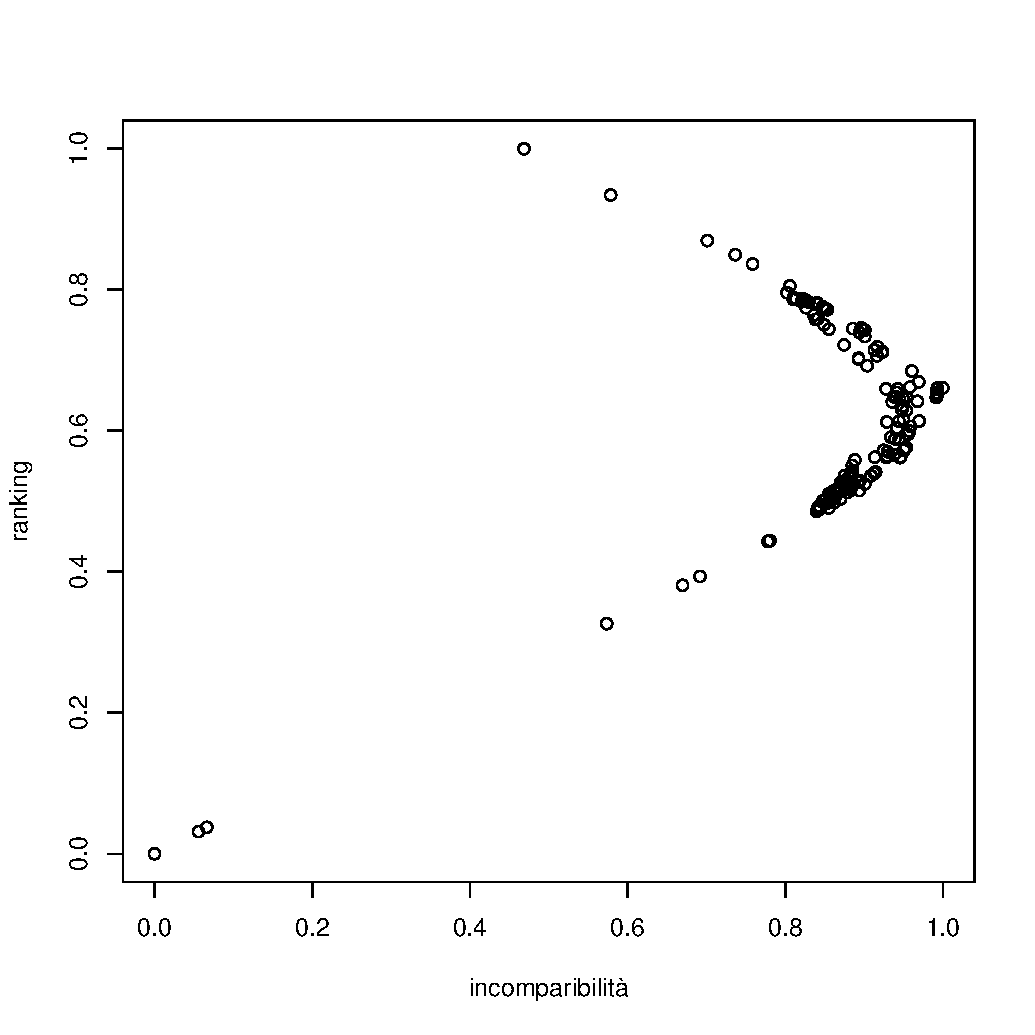
\includegraphics[scale=.5]{plot_incom_eco.pdf}
    \caption{Grafico dell'incomparabilità della dimensione dell'Economia}
\end{figure}

Dal grafico possiamo vedere come la maggior parte dei punti si distribuisce nella fascia medio alta del ranking, indicando che la maggior parte dei paesi ha ottenuto 
dei valori alti nella dimensione economica. Allo stesso modo, è da sottolineare il fatto che la quasi totalità degli stati ha anche alti valori di incomparabilità; 
solo tre paesi infatti hanno un punteggio di incomparabilità minore di 0.4. Questo significa che i valori che vediamo nel ranking finale presentano molta distorsione 
rispetto all'informazione originaria. 
Di conseguenza, osservando il grafico, possiamo affermare che nella dimensione economica la maggior parte degli stati ottiene un alto punteggio, ma è anche presente 
molta distorsione dell'informazione originale. Questo rende molto difficile perciò fare un paragone tra la maggior parte degli stati; alti punteggi di incomparabilità 
indicano che i paesi presentano diversi pattern e sfumatore in questo settore, che vengono in parte perse nella riduzione ad un ranking. Inoltre, anche se due paesi presentano due 
punteggi di incomparabilità simili non significa che essi siano strutturalmente simili$\footnote[17]{Rimoldi Stefania M.L., Arcagni Alberto, Fattore Marco, Terzera Laura, \say{Social and Material Vulnerability of
the Italian Municipalities: Comparing
Alternative Approaches}, 2022[15]  }$; ciò significa che due paesi che hanno ottenuto 
lo stesso punteggio non sono così facilmente comparabili tra loro. 


\newpage

\section{Demografia}

Per la sezione della demografia sono presenti solo i dati del 2021, perciò questa si presenta come la dimensione con il minor numero di osservazioni. In 
aggiunta, i dati della Svizzera, 
al contrario di ciò che accade nelle altre dimensioni, non sono disponibili; di seguito viene presentato il grafico della classifica. \\

\begin{figure}[H]
    \centering
    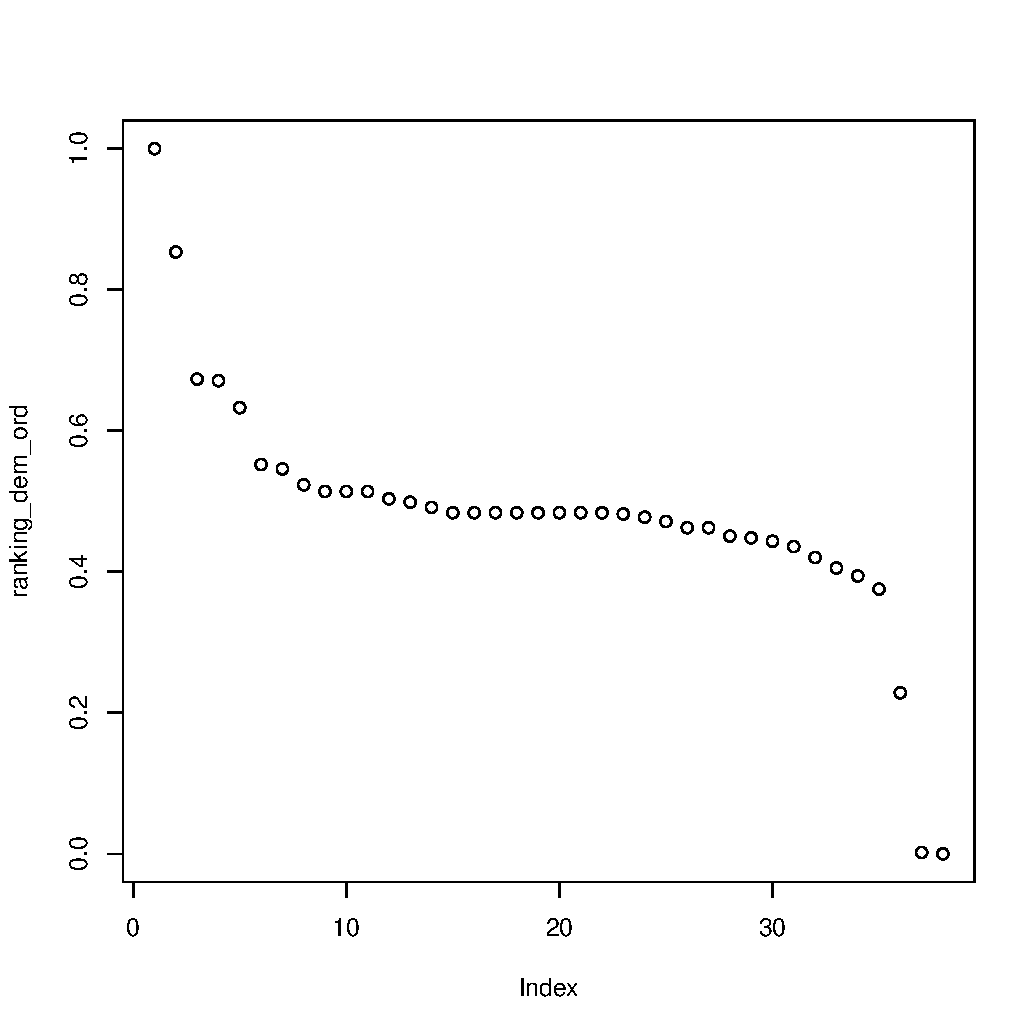
\includegraphics[scale=.5]{ranking_dem_norm.pdf}
    \caption{Grafico della classifica della dimensione demografica}
\end{figure}


Dal grafico possiamo vedere come la maggioranza degli stati hanno un punteggio che varia nell'intervallo [0.40;0.55], con solo cinque paesi che superano questa 
soglia e solo tre paesi assumono un valore minore di 0.35. \\
\\
Di seguito viene riportata la tabella con tutti i punteggi per questa dimensione; 

\begin{table}[h!]
    \centering
    \begin{tabular}{ |l|l|l|  }
        \hline
        \textbf{Posizione} & \textbf{Paese} & \textbf{Punteggio} \\
        \hline
        1° & UK & 1.0000  \\
        \hline
        2° & Netherlands  & 0.8535 \\
        \hline
        3° & Spain  & 0.6731 \\
        \hline
        4° & Portugal  & 0.6709 \\
        \hline
        5° & Israel & 0.6327 \\
        \hline
        6° & Germany & 0.5520\\
        \hline
        7° & Serbia  & 0.5459\\
        \hline
        8° & Ireland  & 0.5232\\
        \hline
        9° & Montenegro  & 0.5139\\
        \hline
        9° & North Macedonia & 0.5139 \\
        \hline
        9° & Ukraine  & 0.5139\\
        \hline
        10° & Slovenia  & 0.5035 \\
        \hline
        11° & Poland  & 0.4986 \\
        \hline
        12° & Slovakia  & 0.4912 \\
        \hline
        13° & Austria  & 0.4837\\
        \hline
        13° & Finland  & 0.4837\\
        \hline
        13° & Iceland  & 0.4837\\
        \hline
        13° & Luxembourg  & 0.4837\\
        \hline
        13° & Malta  & 0.4837\\
        \hline
        13° & Norway  & 0.4837\\
        \hline
        13° & Sweden  & 0.4837\\
        \hline
        13° & Turkey  & 0.4837 \\
        \hline
        14° & Belgium  & 0.4819 \\
        \hline
        15° & EU  & 0.4774 \\
        \hline
        16° & Czechia  & 0.4713 \\
        \hline
        17° & Italy  & 0.4624 \\
        \hline
        18° & Denmark & 0.4623 \\
        \hline
        19° & Cyprus  & 0.4506 \\
        \hline
        20° & Romania  & 0.4480 \\
        \hline
        21° & Lithuania & 0.4433 \\
        \hline
        22° & France  & 0.4357 \\
        \hline
        23° & Hungary  & 0.4202 \\
        \hline
        24° & Greece  & 0.4053 \\
        \hline
        25° & Estonia  & 0.3940\\
        \hline
        26° & Bosnia\&Herzegovina  & 0.3753 \\
        \hline
        27° & Latvia  & 0.2283 \\
        \hline
        28° & Croatia  & 0.0018\\
        \hline
        29° & Bulgaria & 0.0000 \\
        \hline
    \end{tabular}
    \caption{Classifica della dimensione demografica}
    \label{table:1}
\end{table}
\newpage

Anche in questa classifica il paese con un punteggio maggiore appare essere il Regno Unito, subito seguito dai Paesi Bassi e la Spagna. Al settimo posto di questa classifica vi sono 
Montenegro, Nord Macedonia e Ucraina tutti a pari merito. Sempre a pari merito, all'undicesimo posto vi sono otto paesi; Austria, Finlandia, Islanda, Lussemburgo, Malta, Norvegia, 
Svezia e Turchia. L'Italia occupa il quindicesimo posto con un valore poco inferiore a quello della media europea. Agli ultimo due posti, con un punteggio nettamente inferiore
rispetto a quello degli altri paesi troviamo la Croazia e la Bulgaria. 
\\
\\
Come per la dimensione dell'Economia, anche qua viene riportato il grafico che mostra sull'asse delle ascisse delle il punteggio di incomparabilità e sull'asse delle 
ordinate il punteggio ottenuto nella classifica; 

\begin{figure}[H]
    \centering
    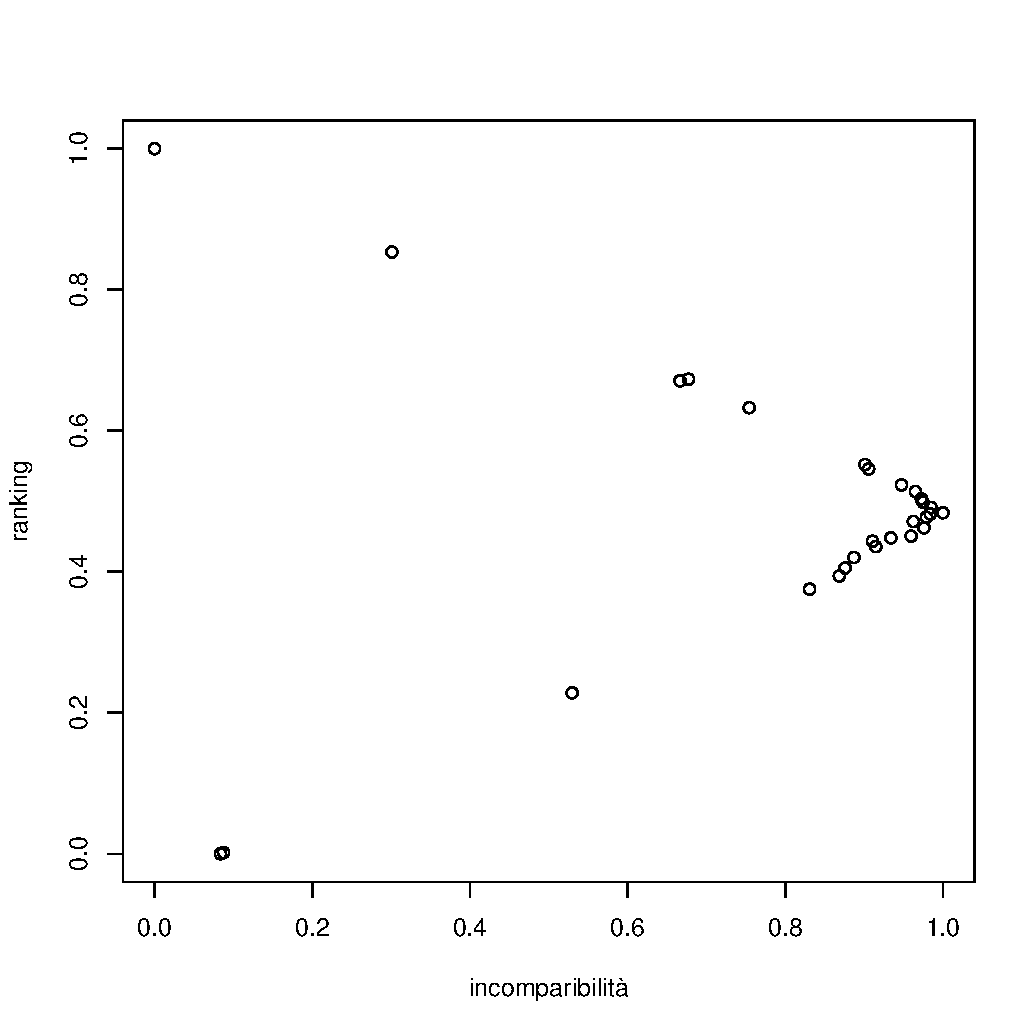
\includegraphics[scale=.5]{plot_incom_dem.pdf}
    \caption{Grafico dell'incomparabilità della dimensione Demografia}
\end{figure}

Come possiamo osservare dal grafico la maggior parte dei paesi ottiene un punteggio medio in questa dimensione, intorno al valore di 0.5. Inoltre, come succedeva anche nel caso della
dimensione economica, anche nella dimensione demografica, la quasi totalità degli stati ottiene punteggio molto elevati di incomparabilità, solo otto paesi infatti, presentano
un valore minore di 0.8. Perciò, in questo caso le conclusioni sono simili a quelle della dimensione precedente; vi è molta perdita di informazione dal sistema di indicatori 
multidimensionale originario alla classifica finale che otteniamo, inoltre non la comparazione tra paesi deve essere effettuata con molta cautela perchè, molti di essi
presentano valori molti distorti. 


\newpage


\section{Istruzione}


Per la dimensione dell'istruzione sono presenti tutti gli stati per gli otto anni di osservazione; di seguito si riporta il grafico. 

\begin{figure}[H]
    \centering
    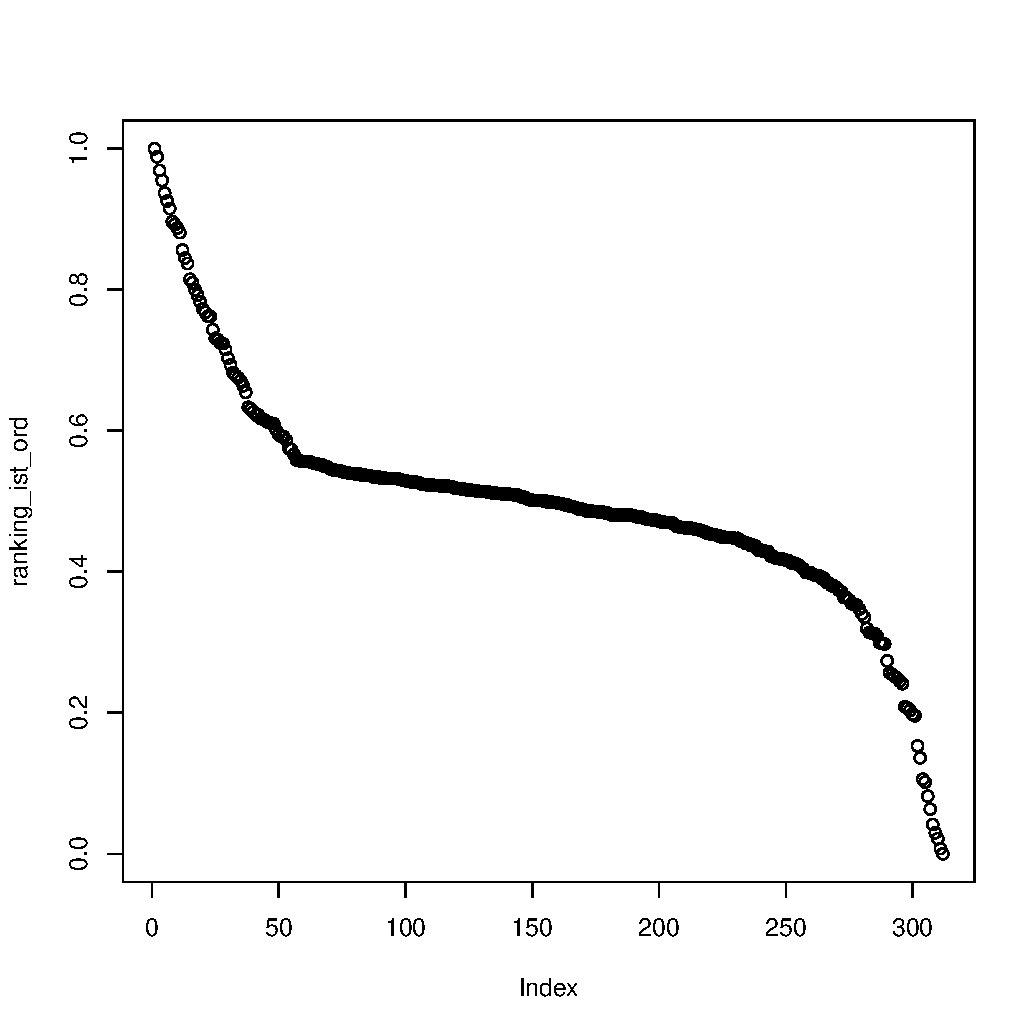
\includegraphics[scale=.5]{ranking_ist_norm.pdf}
    \caption{Grafico della classifica della dimensione Istruzione}
\end{figure}

Come si può osservare dal grafico, la maggior parte degli stati è compresa nell'intervallo [0.30;0.60], con solo pochi paesi che assumono valori al di fuori 
di questo intervallo. Vi è una tendenza crescente per i valori superiori a 0.60, fino ad arrivare ad un massimo di 1; allo stesso modo, vi è
una tendenza decrescente, oltre il valore di 0.40, con solo undici paesi che presentano un valore inferiore a 0.20. \\
\\
Di seguito viene riportata la tabella con tutti i trecentododici elementi della dimensione Istruzione; \\

\setlength\tabcolsep{2pt}
\begin{longtable}[c]{|c|c|c|c|c|c|}
    \hline
    \textbf{Posizione} & \textbf{Paese} & \textbf{Punteggio} & \textbf{Posizione} & \textbf{Paese} & \textbf{Punteggio}\\
    \hline
    1° & UK-2021 & 1.0000 &  13° & Norway-2019 & 0.8449 \\ 
    \hline
    2°	& UK-2020 & 0.9884 &  14° &  Spain-2021 & 0.8372 \\ 
    \hline
    3°	& UK-2019 & 0.9691 &  15° &  UK-2016 & 0.8148\\ 
    \hline
    4°	& Switzerland-2021 & 0.9550 & 16° &  Luxembourg-2020 & 0.8049\\ 
    \hline
    5°	& UK-2018 & 0.9372 & 17° &  Netherlands-2021 & 0.7997\\ 
    \hline
    6°	& Switzerland-2020 & 0.9258 & 18° &  Norway-2018 & 0.7922\\ 
    \hline
    7°	& Norway-2021 & 0.9151 & 19° &  Sweden-2021 & 0.7828\\ 
    \hline
    8°	& UK-2017 & 0.8965  & 20° &   Switzerland-2017 & 0.7728\\ 
    \hline
    9°	& Switzerland-2019 & 0.8923 & 21° &  Sweden-2020 & 0.7678 \\
    \hline
    10° & Luxembourg-2021 & 0.8874 & 22° &  Netherlands-2020 & 0.7624 \\
    \hline
    11° & Norway-2020 & 0.8810 & 23° &  Spain-2020 & 0.7619 \\
    \hline
    12° & Switzerland-2018 & 0.8562 & 24° &  Norway-2017 & 0.7433\\
    \hline
    25° &  Sweden-2019  & 0.7310 & 69° &  Serbia-2020 & 0.5448 \\
    \hline
    26° & Slovenia-2021 & 0.7290 & 70° &  Latvia-2021 & 0.5444\\
    \hline
    27° &  Ireland-2021 & 0.7245 & 71° &  Italy-2021 & 0.5435 \\
    \hline
    28° &   UK-2015 & 0.7236 & 72° &  Ukraine-2015 & 0.5431\\
    \hline
    29° &  Netherlands-2019 & 0.7151 & 73°&  Poland-2021  & 0.5420\\
    \hline
    30° & Slovenia-2019 & 0.7028 & 74° &  Montenegro-2018 & 0.5411 \\
    \hline
    31° & Spain-2019 & 0.6932 & 75°	&  Malta-2019 & 0.5407\\
    \hline
    32° &  Ireland-2020 & 0.6822 & 76°	&  Portugal-2019 & 0.5396\\
    \hline
    33° &  Sweden-2018 & 0.6782 & 77° &  Serbia-2021 & 0.5392\\
    \hline
    34° &  Luxembourg-2019 & 0.6752 & 78° &  Belgium-2019 & 0.5388 \\
    \hline
    35° &  Switzerland-2016 & 0.6710 & 79° &  Belgium-2020 & 0.5384 \\
    \hline
    36° &  Netherlands-2018 & 0.6636 & 80°&  Portugal-2020 & 0.5383 \\
    \hline
    37° &  Norway-2016 & 0.6545 & 81° &  Bosnia\&Herzegovina-2021 & 0.5370  \\
    \hline
    38° &  Sweden-2017 & 0.6334 & 82° &  Greece-2021 & 0.5369\\
    \hline
    39° & Slovenia-2018 & 0.6304 & 83°	&  Romania-2021 & 0.5366 \\
    \hline
    40° & Luxembourg-2018 & 0.6266  & 84° &  Turkey-2017 & 0.5363 \\
    \hline
    41° &  Slovenia-2020 & 0.6222 & 85° &  Ukraine-2020 & 0.5347 \\
    \hline
    42° &  Spain-2018 & 0.6221 & 85° &  Luxembourg-2017 & 0.5347 \\
    \hline
    43° &  Iceland-2020 & 0.6172 & 86° &  Ukraine-2014 & 0.5346 \\
    \hline
    44° &  Iceland-2021 & 0.6160 & 87° &  Turkey-2015 & 0.5333 \\
    \hline
    45° & Portugal-2021 & 0.6137 & 88° &  North Macedonia-2021 & 0.5331  \\
    \hline
    46° &  Netherlands-2017 & 0.6118 & 89° &  Serbia-2018 & 0.5326\\
    \hline
    47° &  Ireland-2019 & 0.6105 & 90° &  Lithuania-2015 & 0.5323 \\
    \hline
    48° &  Slovenia-2017 & 0.6102 & 90° &  Lithuania-2016 & 0.5323 \\
    \hline
    49° &  Iceland-2019 & 0.6007 & 91° &  North Macedonia-2018  & 0.5321 \\
    \hline
    50° &  Sweden-2016 & 0.5947 & 91° &  Spain-2016 & 0.5321 \\
    \hline
    51° &  Iceland-2018 & 0.5919 & 92°	&  Turkey-2016 & 0.5320 \\
    \hline
    52° &  Switzerland-2015 & 0.5916 & 93° &  Ireland-2017 & 0.5309 \\
    \hline
    53° &   UK-2014 & 0.5866 & 94° &  Greece-2020 & 0.5296 \\
    \hline
    54° &  Norway-2015 & 0.5749 & 95° &  Lithuania-2014 & 0.5289 \\
    \hline
    55° &  Ireland-2018 & 0.5734 & 96° &  Estonia-2021 & 0.5279 \\
    \hline
    56° &  Spain-2017 & 0.5667 & 97° &  Germany-2018 & 0.5276 \\
    \hline
    57° &  Serbia-2019 & 0.5584 & 98°	& Slovakia-2020 & 0.5275 \\
    \hline
    58° &  North Macedonia-2019 & 0.5581 & 99° &  Cyprus-2017 & 0.5273 \\
    \hline
    59° &  Netherlands-2016 & 0.5564 & 100° &  Hungary-2021 & 0.5266 \\
    \hline
    60° &  Ukraine-2017  & 0.5563 & 101° &  Denmark-2021 & 0.5248\\
    \hline
    60° &  Germany-2014 & 0.5563 & 102° &  Austria- 2015 & 0.5238 \\
    \hline
    60° &  Germany-2015 & 0.5563 & 103° &  Turkey-2014 & 0.5237 \\
    \hline
    61° &  Germany-2016 & 0.5549 & 104° &  Bosnia\&Herzegovina-2020 & 0.5229 \\
    \hline
    62° &  Ukraine-2018 & 0.5535 & 105° &  Montenegro-2017 & 0.5228 \\
    \hline
    63° & Montenegro-2019 & 0.5531 & 106° &  Cyprus-2016 & 0.5227 \\
    \hline
    64° &  North Macedonia-2020 & 0.5519  & 107° &  France-2021 & 0.5224 \\
    \hline
    65° &  Germany-2017 & 0.5518 & 108° &  Ukraine-2016 & 163.83 \\
    \hline
    66° &  Slovakia-2021 & 0.5493  & 109° &  Montenegro-2020 & 163.64\\
    \hline
    67° &  Sweden-2015 & 0.5489 & 110° &  France-2020 & 0.5222 \\
    \hline
    68° &  Ukraine-2019  & 0.5466 & 111° &  France-2019 & 0.5216 \\
    \hline
    112° &  Austria-2014 & 0.5215 & 158° &  Portugal-2017 & 0.4967 \\
    \hline
    113° &  Serbia-2017 & 0.5213 & 159° &  Denmark-2020 & 0.4960 \\
    \hline
    114° &  Austria- 2018 & 0.5213 & 160° &  Sweden-2014 & 0.4950 \\
    \hline
    115° &  Finland-2019 & 0.5210 & 161° &  Poland-2019 & 0.4944 \\
    \hline
    116° &  Belgium -2017 & 0.5191 & 162° &  Switzerland-2014 & 0.4930 \\
    \hline
    117° &  Latvia-2020 & 0.5186 & 163° &  Malta-2018 & 0.4925 \\
    \hline
    118° &  Turkey-2020 & 0.5181 & 164° &  Czechia-2020 & 0.4910 \\
    \hline
    119° &  Israel-2020 & 0.5173 & 165° &  Montenegro-2016 & 0.4893 \\
    \hline
    120° &  Montenegro-2021 & 0.5171 & 166° & Austria-2017 & 0.4887 \\
    \hline
    121° &  Estonia-2020 & 0.5164 & 167° &  Slovakia-2019 & 0.4886 \\
    \hline
    122° &  Ukraine-2021 & 0.5163 & 168° &  Portugal-2016 & 0.4865 \\
    \hline
    123° &  Spain-2015 & 0.5157 & 169° &  Norway-2014 & 0.4862 \\
    \hline
    124° &  Iceland-2017 & 0.5154 & 170° &  Lithuania-2018 & 0.4858 \\
    \hline
    125° &  North Macedonia-2017 & 0.5147 & 171° &  Denmark-2019 & 0.4857 \\
    \hline
    126° &  Turkey-2019 & 0.5140 & 172° &  Italy-2019 & 0.4855 \\
    \hline
    127° &  Belgium -2021 & 0.5139 & 173° &  Turkey-2021 & 0.4851 \\
    \hline
    128° &  Israel-2017 & 0.5138 & 174° &  Israel-2018 & 0.4848 \\
    \hline
    129° &  Turkey-2018 & 0.5133 & 175° &  Ireland-2016 & 0.4845 \\
    \hline
    130° &  Lithuania-2019 & 0.5128 & 176° &  France-2018 & 0.4832 \\
    \hline
    131° &  Israel-2019 & 0.5119 & 177° &  France-2017 & 0.4831 \\
    \hline
    132° &  Romania-2020 & 0.5114 & 178° &  Austria-2021 & 0.4803 \\
    \hline
    133° &  Malta-2020 & 0.5112 & 178° &  Cyprus-2018 & 0.4803 \\
    \hline
    134° &  Italy-2020 & 0.5109 & 178° &  Cyprus-2019 & 0.4803 \\
    \hline
    135° &  Finland-2021 & 0.5107 & 178° &  Cyprus-2020 & 0.4803 \\
    \hline
    136° & Belgium-2016 & 0.5103 & 178° & Cyprus-2021 & 0.4803 \\
    \hline
    137° &  Belgium-2018 & 0.5099 & 179° &  Poland-2018 & 0.4802 \\
    \hline
    138° & Portugal-2014 & 0.5098 & 180° &  Austria- 2019 & 0.4801 \\
    \hline
    139° &  Cyprus-2014 & 0.5097 & 181° &  Finland-2018 & 0.4799 \\
    \hline
    140° &  Estonia-2019  & 0.5090 & 182° &  Spain-2014 & 0.4780 \\
    \hline
    141° &  Poland-2020 & 0.5089 & 183° &  Serbia-2015 & 0.4780 \\
    \hline
    142° &  Israel-2021 & 0.5075  & 184° &  Germany-2019 & 0.4778 \\
    \hline
    143° &  Israel-2016 & 0.5059 & 185° &  Iceland-2016 & 0.4763 \\
    \hline
    144° &  Belgium-2014 & 0.5056 & 186° &  Greece-2019 & 0.4748 \\
    \hline
    145° &  Austria-2016 & 0.5032 & 187° &  Latvia-2019 & 0.4740 \\ 
    \hline
    146° & Malta-2021 & 0.5023 & 188° &  Luxembourg-2016 & 0.4739 \\
    \hline
    147° &  Portugal-2018 & 0.5013 & 189° &  Luxembourg-2015 & 0.4733 \\
    \hline
    148° &  Belgium-2015 & 0.5012 & 190° &  Italy-2018 & 0.4730 \\
    \hline
    149° &  Cyprus-2015 & 0.5011 & 191° &  Denmark-2018 & 0.4717 \\
    \hline
    150° &  Netherlands-2015 & 0.5010 & 192° &  Slovakia-2018 & 0.4704 \\ 
    \hline
    151° &  Finland-2020 & 0.5006 & 193° &  Slovenia-2015 & 0.4703 \\ 
    \hline
    152° &  Czechia-2019 & 0.5004 & 194° &  Denmark-2014 & 0.4700 \\
    \hline
    153° &  Serbia-2016 & 0.4989 & 195° &  Ireland-2015 & 0.4699 \\
    \hline
    154° &  Portugal-2015 & 0.4988 & 196° &  Montenegro-2015 & 0.4698 \\ 
    \hline
    155° &  Israel-2014 & 0.4984 & 197° &  Slovenia-2014 & 0.4672 \\ 
    \hline
    156° &  Israel-2015 & 0.4982 & 198° &  Luxembourg-2014 & 0.4645 \\
    \hline
    157° & Lithuania-2017 & 0.4975 & 199° &  Czechia-2021 & 0.4637 \\
    \hline
    200° &  Bosnia\&Herzegovina-2019 & 0.4626 & 245° &  Poland-2016 &  0.4095\\
    \hline
    201° &  Hungary-2020 & 0.4626 & 246° &  Finland-2014 &  0.4066\\
    \hline
    202° &  Germany-2020 & 0.4621 &  247° &  Bosnia\&Herzegovina-2017 &  0.4036\\
    \hline
    203° &  Lithuania-2020 & 0.4617 & 248° &  Bulgaria-2021 &  0.3988 \\
    \hline
    204° &  Slovenia-2016 & 0.4616 &  249° &  Czechia-2016 &  0.3985\\
    \hline
    205° &  Lithuania-2021 & 0.4608 &  250° &  Czechia-2018 &  0.3982\\
    \hline
    206° &  Denmark-2016  & 0.4600 & 251° & Hungary-2019 &  0.3959\\
    \hline
    207° & Austria-2020 & 0.4591 & 252° & Czechia-2017 &   0.3948 \\
    \hline
    208° &  Denmark-2017 & 0.4578 & 253° &  Romania-2018 & 0.3947 \\
    \hline
    209° &  Serbia-2014 & 0.4569 & 254° & Latvia-2018 &  0.3909\\
    \hline
    210° &  Iceland-2015 & 0.4545 &  255° &  Poland-2014 &  0.3908 \\
    \hline
    211° &  Romania-2019 & 0.4539 &  256° &  Slovakia-2015 & 0.3850 \\
    \hline
    212° &  Ireland-2014 & 0.4530 & 257° &  North Macedonia-2014 &  0.3839 \\
    \hline
    212° &  EU-2014 & 0.4529 & 258° &  Czechia-2015 &  0.3802 \\ 
    \hline
    213° &  Slovakia-2017 & 0.4512 & 259° &  Italy-2015 &  0.3800 \\ 
    \hline
    214° &  Finland-2017 & 0.4507 & 260° &  Croatia-2020 &  0.3773 \\ 
    \hline
    215° &  Finland-2016 & 0.4489 & 261° &  Estonia-2017 &  0.3737\\ 
    \hline
    216° & North Macedonia-2016 & 0.4488 & 262° &  Malta-2015 & 0.3713 \\ 
    \hline
    217° &  Netherlands-2014 & 0.4487 & 263° &  Greece-2017 &  0.3635 \\ 
    \hline
    218° & Iceland-2014 & 0.4485 &  264° &  Slovakia-2014 & 0.3632 \\ 
    \hline
    219° &  EU-2021 & 0.4481 & 265° &  Estonia-2016 &  0.3599 \\ 
    \hline
    220° &  Malta-2017 & 0.4474 & 266° &  Romania-2017 &  0.3546\\
    \hline
    221° &  Germany-2021 & 0.4473 & 267° &  Czechia-2014 & 0.3532 \\ 
    \hline
    222° &  Poland-2017 & 0.4439 &  268° &  Italy-2014 & 0.3526 \\ 
    \hline
    223° &  Croatia-2021 & 0.4431 & 269° &  Estonia-2015 & 0.3469 \\ 
    \hline
    224° & EU-2018 & 0.4406 & 270° &  Bosnia\&Herzegovina-2016 & 0.3404 \\ 
    \hline
    225° &  France-2016 & 0.4404 & 271° & Romania-2016 & 0.3355 \\ 
    \hline
    226° &  EU-2020 & 0.4377 & 272° &  Malta-2014 & 0.3194 \\
    \hline
    227° & Bosnia\&Herzegovina-2018 & 0.4376 &  273° &  Latvia-2017 & 0.3139 \\ 
    \hline
    228° & EU-2017 & 0.4366  & 274°&  Estonia-2014 & 0.3129 \\ 
    \hline
    229° & Italy-2017 & 0.4309 & 275° &  Bulgaria-2020 &  0.3125 \\ 
    \hline
    230° &  France-2014 & 0.4309 & 276° &  Hungary-2018 & 0.3090 \\
    \hline
    231° & Montenegro-2014 & 0.4292 & 277° &  Bosnia\&Herzegovina-2015 & 0.3085 \\ 
    \hline
    232° &  EU-2019 & 0.4291 & 278° &  Romania-2015 & 0.2993 \\
    \hline
    233° &  France-2015 & 0.4289 & 279° &  Greece-2016 & 0.2983 \\
    \hline
    234° & North Macedonia-2015 & 0.4225 & 280° &  Latvia-2016 & 0.2975\\
    \hline
    235° &  Denmark-2015 & 0.4220 & 281° &  Romania-2014 & 0.2737 \\
    \hline
    236° &  Finland-2015 & 0.4195 & 282° &  Bosnia\&Herzegovina-2014 & 0.2567 \\
    \hline
    237° &  Poland-2015 & 0.4187 & 283° &  Croatia-2019 & 0.2543 \\
    \hline
    238° &  Estonia-2018 & 0.4179 & 284° &  Hungary-2017 & 0.2512 \\
    \hline
    239° &  Italy-2016 & 0.4178 & 285° &  Greece-2015 & 0.2489 \\
    \hline
    240° & Slovakia-2016 & 0.4164 & 286° &  Latvia-2015 & 0.2448 \\
    \hline
    241° & EU-2015 & 0.4161 & 287° &  Croatia-2018 & 0.2411 \\
    \hline
    242° &  EU-2016 & 0.4129 & 288° &  Latvia-2014 & 0.2086 \\
    \hline
    243° &  Malta-2016 & 0.4123 & 289° &  Greece-2014 & 0.2069\\
    \hline
    244° &  Greece-2018 & 0.4112 & 290° &  Bulgaria-2019 & 0.2032 \\
    \hline
\end{longtable}

\begin{table}[h!]
    \centering
    \begin{tabular}{ |l|l|l|  }
        \hline
        \textbf{Posizione} & \textbf{Paese} & \textbf{Punteggio} \\
        \hline
        291° & Hungary-2016 & 0.1980 \\
        \hline
        292° & Hungary-2015 & 0.1958 \\
        \hline
        293° &  Bulgaria-2018 & 0.1750 \\
        \hline
        294° & Croatia-2017 & 0.1530 \\
        \hline
        295° &  Hungary-2014 & 0.1361 \\
        \hline
        296° &  Bulgaria-2017 & 0.1059 \\
        \hline
        297° &  Croatia-2016 & 0.0817 \\
        \hline
        298° &  Croatia-2015 & 0.0633 \\
        \hline
        299° &  Bulgaria-2016 & 0.0414 \\
        \hline
        300° &  Croatia-2014 & 0.0297 \\
        \hline
        301° &  Bulgaria-2015 & 0.0007 \\
        \hline
        302° &  Bulgaria-2014 & 0.0000 \\
        \hline
    \end{tabular}
    \caption{Classifica della dimensione Istruzione}
    \label{table:1}
\end{table}

Anche nella dimensione Istruzione il paese che ottiene il punteggio maggiore e che domina le prime posizioni è il Regno Unito, il quale raggiunge il 
primo posto nel 2021, il secondo nel 2020 ed il terzo nel 2019. Le prime dieci posizioni sono occupate da Regno Unito, Svizzera, Norvegia e Lussemburgo in diversi anni, 
successivamente fino alla quarantesima posizione sono sempre i paesi sopracitati ad occupare queste posizioni, con l'aggiunta di Spagna, Slovenia, Svezia ed Irlanda. 
Come già accenato, la 
maggior parte dei paesi si colloca tra valori di [0.40;0.60], con una media europa molto altalenante nei diversi anni, 
essa infatti raggiunge un massimo nel 2014 con un valore pari a 
0.4529 ed un minimo nel 2016 con un valore pari a 0.4129. L'Italia raggiunge un punteggio massimo nel 2021 con un valore 
pari a 0.5435, 
aggiudicandosi la 71° posizione,
mentre il valore minimo viene raggiunto nel 2014 con un valore pari a 0.3526. Perciò diversi anni l'Italia ha sempre migliorato 
aggiudicandosi posizioni sempre più alte. 
Nelle ultime tredici posizioni vi sono sempre Bulgaria, Croazia ed Ungheria per diversi anni, con il punteggio minimo ottenuto dalla 
Bulgaria nel 2014.
\\
\\
Infine viene mostrato il grafico che mostra l'incomparabilità ed il ranking dei paesi; 

\begin{figure}[H]
    \centering
    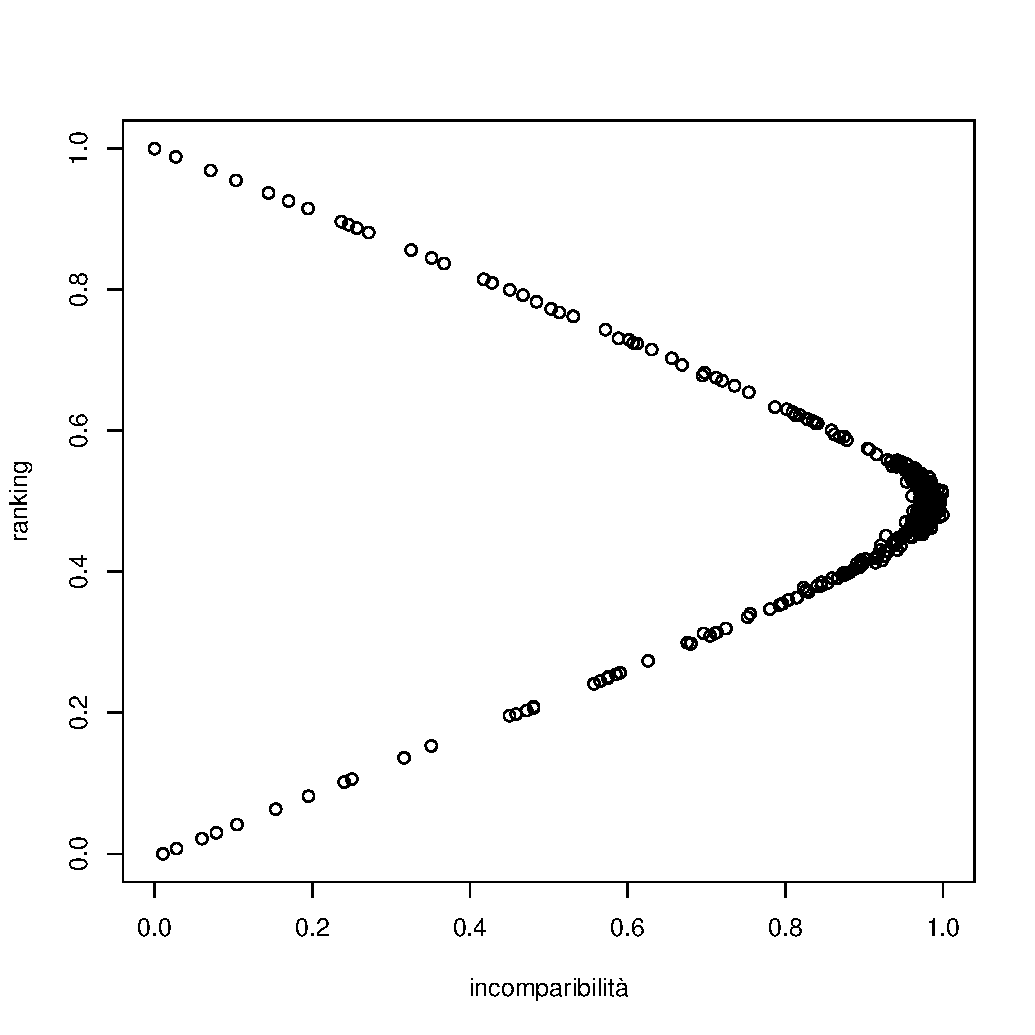
\includegraphics[scale=.5]{plot_incom_ist.pdf}
    \caption{Grafico dell'incomparabilità della dimensione Istruzione}
\end{figure}

A differenza delle altre due dimensioni, la distribuzione dei paesi in questo caso è leggermente diversa; i paesi si dispongono in modo più variegato sul grafico. Molti 
paesi risultano ancora concentrati nei valori medi del ranking e valori alti di incomparabilità, ma molto punti occupano anche altre posizioni; più i punti occupano posizioni
alte o basse nel raking, minore è la loro distorsione. Ciò significa che per i paesi con punteggi medi la distorsione dell'informazione è maggiore, mentre per paesi con
punteggi particolarmente alti o particolarmente bassi la distorsione è molto minore. Questo indica che i punteggi particolarmente alti e quelli particolarmente bassi 
rappresentano in modo più veritiero il fenomeno in studio, rispetto a tutti quei paesi che hanno ottenuto valori medi nel ranking. 


\newpage


\section{Innovazione}


Di seguito viene presentato il grafico che mostra la distribuzione della classifica della dimensione dell'Innovazione; 

\begin{figure}[H]
    \centering
    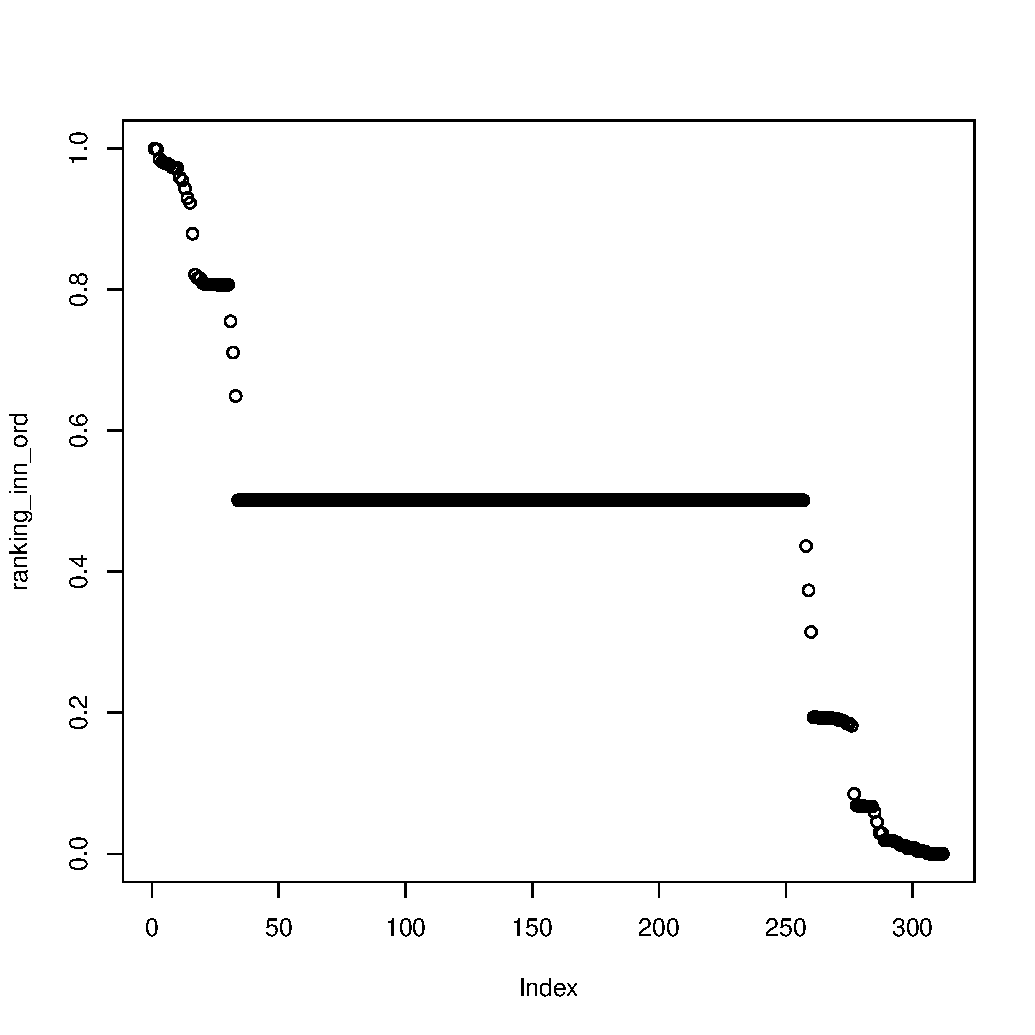
\includegraphics[scale=.5]{ranking_inn_dorm.pdf}
    \caption{Grafico della classifica della dimensione Innovazione}
\end{figure}


Si possono facilmente identificare cinque cluster distinti, che raggruppano la quasi totalità dei paesi. 
Un primo cluster è composto da un insieme di paesi che superano il valore di 0.85. Succesivamente, 
si denota un altro insieme di paesi che assume valori pari a 0.80, il cluster maggiore invece presenta dei valori quasi costanti pari a 
0.50. Infine vi sono altri due cluster;
uno dei quali contiene i paesi che assumono valori pari a 0.18, mentre l'altro è il 
più disomogeneo 
con il valore massimo di 0.15 ed il 
valore minimo di 0. \\

Di seguito viene presentata la tabella contentente la classifica della dimensione Innovazione; 

\setlength\tabcolsep{2pt}
\begin{longtable}[c]{|c|c|c|c|c|c|}
    \hline
    \textbf{Posizione} & \textbf{Paese} & \textbf{Punteggio} & \textbf{Posizione} & \textbf{Paese} & \textbf{Punteggio}\\
    \hline
     1° & Bosnia\&Herzegovina-2014  & 1.0000 &  12° &  Switzerland-2014 & 0.9434 \\ 
    \hline
    2°	& Montenegro-2016 & 0.9991 &  13° &  Ukraine-2020 & 0.9300 \\ 
    \hline
    3°	& Ukraine-2018 & 0.9852 &  14° &  Bulgaria-2014  & 0.9230 \\ 
    \hline
    4°	& Croatia-2017 & 0.9814 & 15° &  Croatia-2018 & 0.8793\\ 
    \hline
    5°	& Croatia-2020  & 0.9795 & 16° & Croatia-2015 & 0.8213 \\ 
    \hline
    6°	& Bulgaria-2017 & 0.9788 & 17° & Luxembourg-2014 & 0.8164 \\ 
    \hline
    7°	& Ukraine-2019 & 0.9766 & 18° & Cyprus-2014 & 0.8163 \\ 
    \hline
    8°	& Bulgaria-2018 & 0.9734  & 19° &  Czechia-2018  & 0.8094 \\ 
    \hline
    9°	& Montenegro-2014 & 0.9726 & 20° & Ukraine-2021 & 0.8080 \\
    \hline
    9° & Montenegro-2015 & 0.9726 & 21° &  Romania-2014 & 0.8075 \\
    \hline
    10° & Croatia-2019 & 0.9591 & 21° &  Romania-2015 & 0.8075 \\
    \hline
    11° & Croatia-2016 & 0.9549 & 21° & Romania-2016 & 0.8075 \\
    \hline
    21° & Latvia-2018  & 0.8075 & 27° &  Bosnia\&Herzegovina-2019  & 0.5014 \\
    \hline
    22° & Latvia-2020 & 0.8071 & 27° &  Bosnia\&Herzegovina-2020  & 0.5014\\
    \hline
    23° &  EU-2014 & 0.8070 & 27° & Bosnia\&Herzegovina-2021 & 0.5014\\
    \hline
    23° &  EU-2015 & 0.8070 & 27° & Bulgaria-2015 & 0.5014\\
    \hline
    23° & EU-2016 & 0.8070 & 27° & Bulgaria-2016  & 0.5014 \\
    \hline
    23° & EU-2017  & 0.8070 & 27° & Bulgaria-2019 & 0.5014\\
    \hline
    24° & Latvia-2017 & 0.7552 & 27° & Bulgaria-2020 & 0.5014\\
    \hline
    25° &  Montenegro-2017 & 0.7109 & 27°	&  Bulgaria-2021 & 0.5014\\
    \hline
    26° &  Croatia-2014 & 0.6492 & 27° &  Croatia-2021 & 0.5014\\
    \hline
    27° &  Switzerland-2017 & 0.5014 & 27° & Cyprus-2016  & 0.5014 \\
    \hline
    27° &  Switzerland-2018  & 0.5014 & 27° & Cyprus-2017 & 0.5014 \\
    \hline
    27° &  Switzerland-2019 & 0.5014 & 27°& Cyprus-2018 & 0.5014 \\
    \hline
    27° &  Switzerland-2020 & 0.5014 & 27° &  Cyprus-2019 & 0.5014  \\
    \hline
    27° &  Switzerland-2021 & 0.5014 & 27° & Cyprus-2020 & 0.5014 \\
    \hline
    27° & Turkey-2014 & 0.5014 & 27° & Cyprus-2021  & 0.5014\\
    \hline
    27° & Turkey-2015  & 0.5014  & 27° &  Czechia-2014 & 0.5014 \\
    \hline
    27° &  Turkey-2016 & 0.5014 & 27° & Czechia-2015 & 0.5014\\
    \hline
    27° &  Turkey-2017 & 0.5014 & 27° &  Czechia-2016 & 0.5014 \\
    \hline
    27° & Turkey-2018 & 0.5014 & 27° &  Czechia-2017 & 0.5014 \\
    \hline
    27° &  Turkey-2019 & 0.5014 & 27° & Czechia-2019  & 0.5014\\
    \hline
    27° & Turkey-2020  & 0.5014 & 27° & Czechia-2020 & 0.5014 \\
    \hline
    27° &  Turkey-2021 & 0.5014 & 27° &  Czechia-2021 & 0.5014 \\
    \hline
    27° &  Ukraine-2014 & 0.5014 & 27° & Denmark-2021 & 0.5014 \\
    \hline
    27° & Ukraine-2015 & 0.5014& 27° & Estonia-2014 & 0.5014\\
    \hline
    27° &  Ukraine-2016 & 0.5014 & 27° & Estonia-2015  & 0.5014 \\
    \hline
    27° &  Ukraine-2017  & 0.5014 & 27° & Estonia-2016 & 0.5014 \\
    \hline
    27° &  UK-2014 & 0.5014 & 27° & Estonia-2017 & 0.5014 \\
    \hline
    27° & UK-2015 & 0.5014 & 27° & Estonia-2018 & 0.5014 \\
    \hline
    27° & UK-2016 & 0.5014 & 27° &  Estonia-2019 & 0.5014 \\
    \hline
    27° & UK-2017 & 0.5014 & 27° & Estonia-2020  & 0.5014\\
    \hline
    27° & Austria-2014  & 0.5014 & 27° & Estonia-2021 & 0.5014\\
    \hline
    27° & Austria-2015 & 0.5014 & 27° & EU-2018 & 0.5014 \\
    \hline
    27° &  Austria-2016 & 0.5014 & 27°	& EU-2019 & 0.5014 \\
    \hline
    27° &  Austria-2017 & 0.5014 & 27° &  EU-2020 & 0.5014\\
    \hline
    27° & Austria-2018 & 0.5014 & 27° &  EU-2021  & 0.5014 \\
    \hline
    27° &  Austria-2019  & 0.5014& 27° &  France-2014 & 0.5014 \\
    \hline
    27° &  Austria-2020 & 0.5014 & 27° & France-2015 & 0.5014 \\
    \hline
    27° & Austria-2021 & 0.5014 & 27° &  France-2016 & 0.5014 \\
    \hline
    27° &  Belgium-2014 & 0.5014 & 27° & France-2017 & 0.5014 \\
    \hline
    27° &  Belgium-2015 & 0.5014 & 27° & France-2018  & 0.5014 \\
    \hline
    27° & Belgium-2016  & 0.5014 & 27° &  France-2019 & 0.5014 \\
    \hline
    27° &  Belgium-2017 & 0.5014  & 27° &  France-2020 & 0.5014 \\
    \hline
    27° & Belgium-2018 & 0.5014 & 27° & France-2021 & 0.5014 \\
    \hline
    27° &  Belgium-2019 & 0.5014  & 27° &  Germany-2019 & 0.5014 \\
    \hline
    27° &  Belgium-2020 & 0.5014 & 27° &  Germany-2020  & 0.5014 \\
    \hline
    27° &  Belgium-2021  & 0.5014 & 27° &  Greece-2014 & 0.5014 \\
    \hline
    27° &  Greece-2015 & 0.5014 & 27° & Latvia-2019 & 0.5014 \\
    \hline
    27° &  Greece-2016 & 0.5014 & 27° & Latvia-2021  & 0.5014 \\
    \hline
    27° &  Greece-2017 & 0.5014 & 27° & Lithuania-2014 & 0.5014 \\
    \hline
    27° &  Greece-2018  & 0.5014 & 27° & Lithuania-2015 & 0.5014 \\
    \hline
    27° &  Greece-2019 & 0.5014 & 27° & Lithuania-2016 & 0.5014 \\
    \hline
    27° &  Greece-2020 & 0.5014 & 27° & Lithuania-2017 & 0.5014 \\
    \hline
    27° &  Greece-2021 & 0.5014 & 27° & Lithuania-2018  & 0.5014 \\
    \hline
    27° &  Hungary-2014 & 0.5014  & 27° & Lithuania-2019 & 0.5014 \\
    \hline
    27° & Hungary-2015  & 0.5014 & 27° & Lithuania-2020 & 0.5014 \\
    \hline
    27° &  Hungary-2016 & 0.5014 & 27° & Lithuania-2021 & 0.5014 \\
    \hline
    27° &  Hungary-2017 & 0.5014 & 27° & Luxembourg-2015 & 0.5014 \\
    \hline
    27° & Hungary-2018 & 0.5014 & 27° & Luxembourg-2019  & 0.5014 \\
    \hline
    27° &  Hungary-2019 & 0.5014 & 27° & Luxembourg-2020 & 0.5014 \\
    \hline
    27° & Hungary-2020  & 0.5014 & 27° & Malta-2014 & 0.5014 \\
    \hline
    27° &  Iceland-2014 & 0.5014 & 27° &  Malta-2015 & 0.5014\\
    \hline
    27° &  Iceland-2015 & 0.5014 & 27° & Malta-2016 & 0.5014\\
    \hline
    27° &  Iceland-2016 & 0.5014 & 27° & Malta-2017  & 0.5014 \\
    \hline
    27° &  Iceland-2017  & 0.5014  & 27° & Malta-2018 & 0.5014 \\
    \hline
    27° & Iceland-2018 & 0.5014 & 27° & Malta-2019 & 0.5014 \\
    \hline
    27° & Iceland-2019 & 0.5014 & 27° & Malta-2020 & 0.5014 \\
    \hline
    27° & Iceland-2020 & 0.5014 & 27° & Malta-2021 & 0.5014 \\
    \hline
    27° &  Iceland-2021 & 0.5014 & 27° & Montenegro-2018  & 0.5014 \\
    \hline
    27° & Ireland-2014  & 0.5014 & 27° & Montenegro-2019 & 0.5014 \\
    \hline
    27° & Ireland-2015 & 0.5014 & 27° & Montenegro-2020 & 0.5014 \\
    \hline
    27° & Ireland-2016 & 0.5014 & 27° & Montenegro-2021 & 0.5014 \\
    \hline
    27° & Ireland-2017 & 0.5014 & 27° & Netherlands-2014 & 0.5014 \\
    \hline
    27° & Ireland-2018 & 0.5014 & 27° & Netherlands-2015  & 0.5014 \\
    \hline
    27° &  Ireland-2019  & 0.5014 & 27° & Netherlands-2016 & 0.5014 \\
    \hline
    27° &  Ireland-2020 & 0.5014 & 27° & North Macedonia-2014 & 0.5014 \\
    \hline
    27° & Ireland-2021 & 0.5014 & 27° & North Macedonia-2015 & 0.5014 \\
    \hline
    27° &  Israel-2014 & 0.5014 & 27° & North Macedonia-2016 & 0.5014 \\
    \hline
    27° & Israel-2015 & 0.5014 & 27° & North Macedonia-2017  & 0.5014\\
    \hline
    27° & Israel-2016  & 0.5014 & 27° & North Macedonia-2018 & 0.5014 \\
    \hline
    27° & Israel-2017 & 0.5014 & 27° & North Macedonia-2019 & 0.5014 \\ 
    \hline
    27° & Israel-2018 & 0.5014 & 27° & North Macedonia-2020 & 0.5014 \\
    \hline
    27° & Israel-2019 & 0.5014 & 27° & North Macedonia-2021 & 0.5014 \\
    \hline
    27° &  Israel-2020 & 0.5014 & 27° & Norway-2014  & 0.5014 \\
    \hline
    27° &  Israel-2021  & 0.5014 & 27° & Norway-2015 & 0.5014 \\
    \hline
    27° & Italy-2014 & 0.5014 & 27° & Norway-2016 & 0.5014 \\ 
    \hline
    27° & Italy-2015 & 0.5014 & 27° & Norway-2017 & 0.5014 \\ 
    \hline
    27° &  Italy-2016 & 0.5014 & 27° & Norway-2018 & 0.5014 \\
    \hline
    27° & Italy-2017 & 0.5014 & 27° & Poland-2014  & 0.5014 \\
    \hline
    27° &  Italy-2018  & 0.5014 & 27° & Poland-2015 & 0.5014 \\ 
    \hline
    27° &  Italy-2019 & 0.5014 & 27° & Poland-2016 & 0.5014 \\ 
    \hline
    27° &  Italy-2020 & 0.5014 & 27° & Poland-2017 & 0.5014\\
    \hline
    27° & Italy-2021 & 0.5014 & 27° & Poland-2018 & 0.5014 \\
    \hline
    27° & Poland-2019  & 0.5014 & 27° & Spain-2020 & 0.5014 \\
    \hline
    27° & Poland-2020 & 0.5014 & 27° & Spain-2021 & 0.5014 \\
    \hline
    27° & Poland-2021 & 0.5014 &  28° & Latvia-2016 & 0.4364 \\
    \hline
    27° & Portugal-2014 & 0.5014 & 29° & Latvia-2015 & 0.3736 \\
    \hline
    27° & Portugal-2015 & 0.5014 &  30° & Latvia-2014  & 0.3146 \\
    \hline
    27° & Portugal-2016  & 0.5014 &  31° & Finland-2018 & 0.1936 \\
    \hline
    27° & Portugal-2017 & 0.5014 & 31° & Germany-2018  & 0.1936 \\
    \hline
    27° & Portugal-2018 & 0.5014 & 32° & Bosnia\&Herzegovina-2015  & 0.1931 \\
    \hline
    27° & Portugal-2019 & 0.5014 & 32° & Bosnia\&Herzegovina-2016  & 0.1931 \\
    \hline
    27° & Portugal-2020 & 0.5014 & 32° & Bosnia\&Herzegovina-2017  & 0.1931 \\
    \hline
    27° & Portugal-2021  & 0.5014 &  32° & Bosnia\&Herzegovina-2018 & 0.1931 \\
    \hline
    27° & Romania-2017 & 0.5014 &  33° & UK-2018 & 0.1929 \\
    \hline
    27° & Romania-2018 & 0.5014 & 33° & Finland-2017 & 0.1929 \\
    \hline
    27° & Romania-2019 & 0.5014 & 34° & Finland-2014 & 0.1919 \\ 
    \hline
    27° & Romania-2020 & 0.5014 & 34° & Germany-2014  & 0.1919 \\ 
    \hline
    27° & Romania-2021  & 0.5014 & 35° & Switzerland-2015 & 0.1894  \\ 
    \hline
    27° & Serbia-2014 & 0.5014 & 35° & Switzerland-2016 & 0.1894 \\ 
    \hline
    27° & Serbia-2015 & 0.5014 & 36° & Sweden-2014 & 0.1879 \\ 
    \hline
    27° & Serbia-2016 & 0.5014& 37° & Cyprus-2015 & 0.1848 \\ 
    \hline
    27° & Serbia-2017 & 0.5014 &  37° & Luxembourg-2016  & 0.1848 \\ 
    \hline
    27° & Serbia-2018  & 0.5014 & 38° & Sweden-2019 & 0.1816 \\ 
    \hline
    27° & Serbia-2019 & 0.5014 & 39° & Germany-2017 & 0.0849 \\
    \hline
    27° & Serbia-2020 & 0.5014 & 40° & Denmark-2017 & 0.0687 \\ 
    \hline
    27° & Serbia-2021 & 0.5014 &  41° & Denmark-2014 & 0.0676 \\ 
    \hline
    27° & Slovakia-2014 & 0.5014 & 42° & Finland-2020  & 0.0675 \\ 
    \hline
    27° & Slovakia-2015  & 0.5014& 42° & Finland-2021 & 0.0675 \\ 
    \hline
    27° & Slovakia-2016 & 0.5014 & 43° & Finland-2015 & 0.0672 \\ 
    \hline
    27° & Slovakia-2017 & 0.5014 & 43° & Germany-2015 & 0.0672 \\
    \hline
    27° & Slovakia-2018 & 0.5014 &  44° & UK-2019 & 0.0671 \\ 
    \hline
    27° & Slovakia-2019 & 0.5014 & 45° & Sweden-2015  & 0.0593 \\ 
    \hline
    27° & Slovakia-2020  & 0.5014& 46° & Sweden-2020 & 0.0452 \\ 
    \hline
    27° & Slovakia-2021 & 0.5014 & 47° & Denmark-2020 & 0.0295 \\
    \hline
    27° & Slovenia-2014 & 0.5014 & 48° & Finland-2019 & 0.0294 \\ 
    \hline
    27° & Slovenia-2015 & 0.5014 & 49° & Denmark-2018 & 0.0292 \\
    \hline
    27° & Slovenia-2016 & 0.5014 & 49° & Denmark-2015  & 0.0292 \\
    \hline
    27° & Slovenia-2017  & 0.5014 & 50° & Finland-2016 & 0.0192 \\
    \hline
    27° & Slovenia-2018 & 0.5014 & 50° & Germany-2016 & 0.0192 \\
    \hline
    27° & Slovenia-2019 & 0.5014 & 51° & Sweden-2021 & 0.0191 \\
    \hline
    27° & Slovenia-2020 & 0.5014 & 52° & UK-2020 & 0.0190 \\
    \hline
    27° & Slovenia-2021 & 0.5014 & 53° & Germany-2021  & 0.0188 \\
    \hline
    27° & Spain-2014  & 0.5014 & 54° & Denmark-2016 & 0.0175 \\
    \hline
    27° & Spain-2015 & 0.5014 & 55° & Denmark-2019 & 0.0161 \\
    \hline
    27° & Spain-2016 & 0.5014 & 56° & Netherlands-2019 & 0.0129 \\
    \hline 
    27° & Spain-2017 & 0.5014 & 56° & Netherlands-2020 & 0.0129 \\
    \hline
    27° & Spain-2018 & 0.5014 & 56° & Netherlands-2021  & 0.0129 \\
    \hline
    27° & Spain-2019  & 0.5014 & 56° & Sweden-2016 & 0.0129 \\
    \hline
\end{longtable}

\begin{table}[h!]
    \centering
    \begin{tabular}{ |l|l|l|  }
        \hline
        \textbf{Posizione} & \textbf{Paese} & \textbf{Punteggio} \\
        \hline
        57° & Norway-2019 & 0.0037 \\
        \hline
        57° & Norway-2020 & 0.0037 \\
        \hline
        57° & Norway-2021 & 0.0037 \\
        \hline
        58° & UK-2021  & 0.0031 \\
        \hline
        59° & Luxembourg-2017 & 0.0004 \\
        \hline
        60° & Netherlands-2017 & 0.0000 \\
        \hline
        60° & Netherlands-2018 & 0.0000 \\
        \hline
        60° & Sweden-2017 & 0.0000 \\
        \hline
        60° & Sweden-2018  & 0.0000 \\
        \hline
        60° & Luxembourg-2018 & 0.0000 \\
        \hline
        60° & Luxembourg-2021  & 0.0000 \\
        \hline
    \end{tabular}
    \caption{Classifica della dimensione Innovazione}
    \label{table:1}
\end{table}


In questa classifica possiamo vedere come i paesi che occupano le prime posizioni sono quelli che, in tutte le altre dimensioni, occupano 
gli 
ultimi posti come Bosnia ed 
Erzegovina, Montenegro, Croazia e Bulgaria, ad eccezione però dell'Ucraina, la quale occupava anche le prime posizioni delle dimensioni
Economia e Demografia. Si nota come
la media europea negli anni 2014, 2015, 2016 e 2017 sia sempre uguale e pari a 0.8070, mentre negli altri anni occupa, come la maggior
parte dei paesi,
la ventisettesima posizione con un valore pari a 0.5014. Come si evidenziava anche dal grafico infatti, quasi tutti i paesi occupano la 
ventisettesima posizione con un 
punteggio pari a 0.5014. In particolare, si denota anche come, in questa posizione spesso si trovano gli stessi paesi per molti anni 
consecutivi; questo significa che 
per diversi stati non vi è nè 
un peggioramento, nè un miglioramento. Questo fa della dimensione Innovazione, la più statistica tra tutte le dimensioni; significa 
che i paesi non migliorano nè peggiorano, semplicemente hanno la stessa performance per tutti gli anni. Da questo deduciamo come la 
dimensione dell'innovazione sia quella in 
cui sono necessari maggiori incentivi per promuovere la crescita nei vari paesi europei in questo settore. \\
Possiamo anche notare come stati che tradizionalmente hanno alte perfomance, si trovino invece tra le ultime posizioni di questa classifica. Infatti, paesi 
come Norvegia, Regno
Unito, Lussemburgo, Paesi Bassi e Svezia sono gli ultimi paesi di questa classifica classificandosi al sessantesimo posto con un punteggio
quasi pari a zero. \\
L'Italia, come la maggior parte dei paesi si trova nella ventisettesima posizione con un punteggio pari a 
0.5014 per tutti e otto gli anni. 
\\
\\
Succesivamente, viene presentato il grafico che mostra punteggio di incomparabilità e ranking; 

\begin{figure}[H]
    \centering
    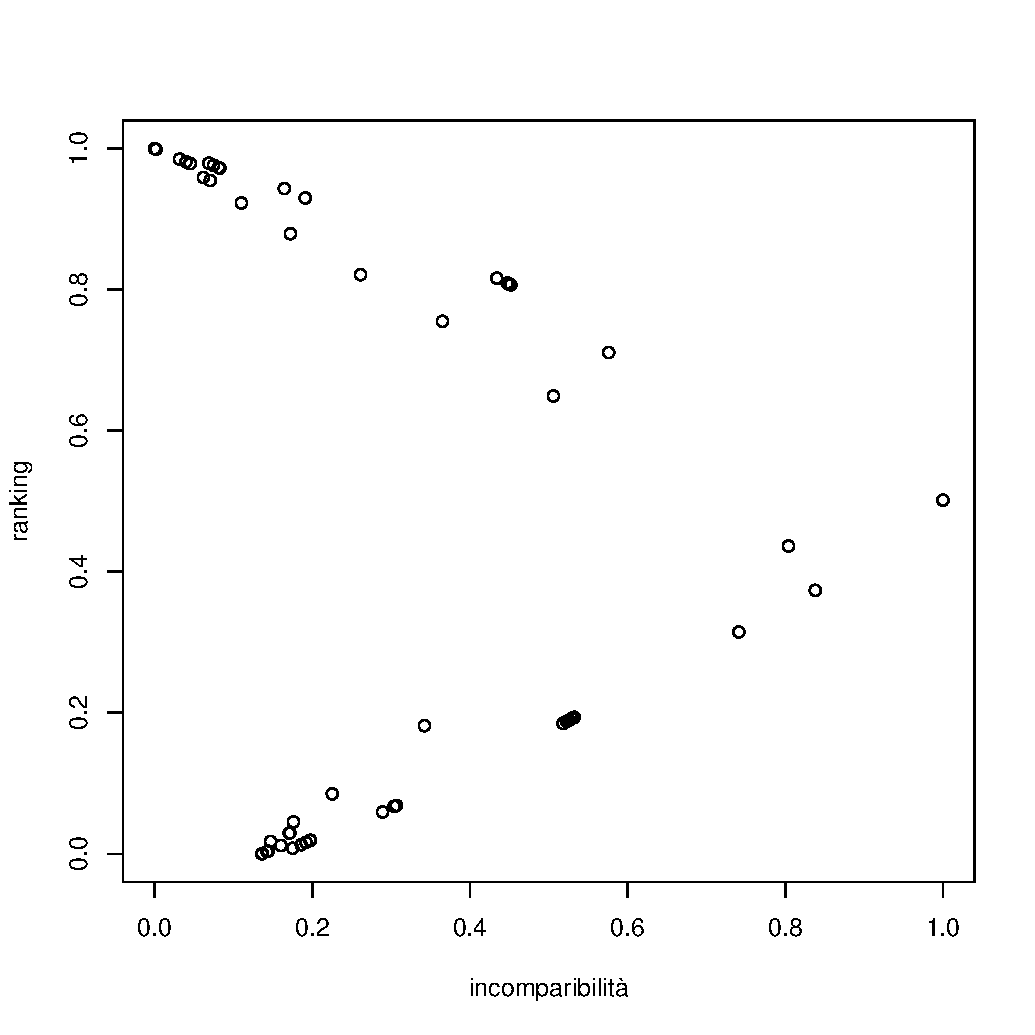
\includegraphics[scale=.5]{plot_incom_inn.pdf}
    \caption{Grafico dell'incomparabilità della dimensione Innovazione}
\end{figure}

Anche per questa dimensione la distribuzione dei punti è differente da quella delle altre dimensioni; sono pochissimi i paesi che ottengono 
un valore medio nel ranking, in 
particolare solo un paese raggiunge il valore 0.5 e corrisponde anche al paese con massima distorsione. Come sottolineato per la dimensione
dell'Istruzione, anche in questo
caso i paesi con valori del ranking particolarmente alti o bassi presentano minore distorsione, mentre più il valore ottenuto nel punteggio 
si avvicina al valore di 0.5, 
maggiormente cresce la distorsione. 

\newpage 

\section{Considerazioni finali}

Alla luce dei risultati presentati precedentemente possiamo affermare che la dimensione dell'Innovazione è quella in cui i paesi emergenti, e 
che solitamente si trovano nelle ultime posizioni nelle altre dimensioni, come Bosnia ed Erzegovina, Croazia, Bulgaria e Montenegro,
hanno le migliori perfomance, mentre i paesi che tradizionalmente 
sono conosciuti come i paesi più benestanti, come Regno Unito, Norvegia, Svezia e Svizzera, e che si trovano quasi sempre in alte posizioni
delle classifiche, sono quelli che stanno 
presentando un minor sforzo nella dimensione dell'Innovazione. Questo può essere dovuto al fatto che questi paesi, perfomando molto bene 
in molto settori abbiano meno incentivi, rispetto ad altri, di innovarsi e presentarsi come più competitivi a livello europeo mentre 
i paesi emergenti hanno un maggior incentivo all'innovazione. 
Inoltre nella dimensione dell'Innovazione, come in quella dell'Istruzione
i paesi che ottengono valori particolarmente bassi o particolarmente alti nel ranking presentano una minor perdita di informazione rispetto a quei paesi 
che ottengono punteggi medi. Al 
contrario, invece delle dimensioni di Economia e Demografia, dove nonostante molti paesi raggiungano punteggi molti simili, le comparazioni hanno una minor
ragion d'essere, alla luce dei punteggi di incomparabilità ottenuti dagli stati e questo porta comparazioni tra stati più difficili e 
meno intuitive, con risultati che vanno letti ed analizzati tramite un'ottica più attenta e che va oltre un semplice confronto delle 
posizioni ottenute nella classifica. \\
\\
In conclusione possiamo affermare che, ad eccezione della dimensione Innovazione, sono i paesi del nord Europa ad occupare quasi sempre 
le posizioni più alte nelle classifiche, con una particolare menzione al Regno Unito che domina sia la dimensione economica che quella 
dell'istruzione. Inoltre sia la dimensione economica che quella dell'innovazione sono le dimensioni maggiormente statiche, con molti stati 
che per diversi anni consecutivi ottengono lo stesso punteggio. Questo può suggerire, come in queste due dimensioni ci sia bisogno di 
particolari politiche in modo da incetivare maggiormente gli stati a migliorare in questi campi. La dimensione demografica, inoltre, 
sottolinea come Croazia e Bulgaria siano i paesi che necessitano di politiche a favore della natalità, con la Bulgaria che sta vivendo 
un vero e proprio crollo demografico; risulta che dal 1989 abbia perso il 10\% della sua popolazione$\footnote[18]{ National Statistical Instite of Bulgaria \url{https://www.nsi.bg/en/content/2920/population-demography-migration-and-projections[16]}}$. 
\\
\\
L'Italia non presenta delle perfomance particolarmente alte in nessuna categoria; solitamente si trova nella media insieme alla maggioranza 
dei paesi. Nella dimensione Innovazione occupa, per tutti gli anni, il ventisettesimo posto insieme alla maggioranza dei paesi; il nostro 
paese come molti altri sembra molto statico in questa dimensione. Nella dimensione demografica l'Italia si colloca poco al di sotto della 
media europea, mentre nell'istruzione vi è stato un progressivo miglioramento, con la miglior perfomance ottenuta nel 2021. Nella dimensione
economica l'Italia ha un andamento molto altalentante e poco stabile; ottiene il punteggio migliore nel 2014 per poi raggiungere sempre posizione
più basse negli anni successivi, con un minimo nel 2017.  
\\
\\
Questi risultati, che sono in linea con quelli di più autorevoli istituzioni come l'Eurostat, si presentano come uno strumento per poter 
comprendere in modo più approfondito e completo la competitività in Europa, con un'attenzione posta anche alle differenze dei diversi stati. 



\afterpage{\blankpage}

\newpage


\cleardoublepage
\phantomsection
\addcontentsline{toc}{chapter}{\listfigurename}
\listoffigures

\newpage

\addcontentsline{toc}{chapter}{Bibliografia e sitografia}
\begin{thebibliography}{9}

    \bibitem{lamport94}
      Word Economic Forum
      \url{https://www.weforum.org/agenda/2016/09/what-is-competitiveness/}
    \bibitem{lamport94}
      Hanna Shvindina,
      \textit{Economic Competitiveness: An Overview of Multilevel Concept},
      2022
      \url{https://link.springer.com/referenceworkentry/10.1007/978-3-319-95726-5_63}
    \bibitem{lamport94}
      Biografia di Helmut Hasse,
      \url{https://mathshistory.st-andrews.ac.uk/Biographies/Hasse/}
    \bibitem{lamport94}
      Tim Roughgarden, Gregory Valiant, 
      \textit{The Singular Value Decomposition (SVD) and Low-Rank Matrix Approximations}, 2022
      \url{https://web.stanford.edu/class/cs168/l/l9.pdf}
    \bibitem{lamport94}
       Alberto Arcagni, Marco Fattore 
      \textit{Posetic Tools in the Social Sciences: A Tutorial Exposition}, 2021
      \url{https://link.springer.com/chapter/10.1007/978-3-030-59683-5_15}
    \bibitem{lamport94}
      Sito personale di Hadley Alexander Wickham
     \url{https://hadley.nz/}
    \bibitem{lamport94}
     GitHub di Romain Fracois
     \url{https://github.com/romainfrancois}
    \bibitem{lamport94}
     GitHub di Pablo Casas
     \url{https://github.com/pablo14}
    \bibitem{lamport94}
     Sito personale di Alberto Arcagni
     \url{https://albertoarcagni.github.io/}
    \bibitem{lamport94}
     Sito personale di David Schoch 
     \url{https://mr.schochastics.net/}
    \bibitem{lamport94}
     Dati EIS
     \url{https://ec.europa.eu/research-and-innovation/en/statistics/performance-indicators/european-innovation-scoreboard/eis}
    \bibitem{lamport94}
     European Innovation Scoreboard Methodology Report 2021 
     \url{https://www.eustat.eus/elementos/European-Innovation-Scoreboard-2021-Methodology-Report/inf0019111_c.pdf}
    \bibitem{lamport94}
     Definizione di economia
     \url{https://it.wikipedia.org/wiki/Economia}
    \bibitem{lamport94}
     Definizione di demografia
     \url{https://www.britannica.com/dictionary/demography}
    \bibitem{lamport94}
     Stefania M.L. Rimoldi, Alberto Arcagni, Marco Fattore, Laura Terzera
     \textit{Social and Material Vulnerability of the Italian Municipalities: Comparing Alternative Approaches},
     2022
     \url{https://link.springer.com/article/10.1007/s11205-020-02330-x}
    \bibitem{lamport94}
     National Statistical Institute of Bulgaria 
     \url{https://www.nsi.bg/en/content/2920/population-demography-migration-and-projections}
\end{thebibliography}

\end{document}



